\clearpage
\section{Event selection and cut optimization}
\label{tW_Eventselection}
The selection of the events to be used for our search is done in two steps which are explained in the following sections.
\subsection{Event selection (step 1)}
\label{step1_selection}
At the first step, we focus on selecting events by requiring trigger and lepton selection. Events should fire one of the triggers summarized in Table \ref{tab:trigger}.
At least 1 pair of opposite charge leptons with invariant mass $>$ 20 GeV is required while leading lepton should have $P_{T}$ $>$ 25 GeV.
The first two selected leptons which are sorted due to the $P_{T}$ should have same flavor opposite sign. If the two highest $P_{T}$ leptons are different flavor (e.g. $e\mu$ event) or same sign, event is rejected.
The events are divided in the ee and $\mu\mu$ channels according to the flavours of the two leptons with the highest $P_{T}$
and are further categorised in different bins depending on the number of jets (``n-jets'') in the final state and the number of them which are b-tagged (``m-tags'').
The largest number of  tW events is expected in the category with exactly one  b-tagged jet (1-jet,1-tag) followed by the category with two jets, one of which being a  b jet (2-jets,1-tag). Events in the categories with more than  two jets and exactly two b-tagged jets  are dominated by $\ttbar$ process ($\geq$2-jets,2-tags).

%Some distributions for Data/MC comparison after this step are shown in figures \ref{fig:step1_leading_lepton1}-\ref{fig:step1_Nvtx_jet_bjet}.
%In Figure \ref{fig:step1_MET_phi}, one can see that the  Data/MC agreement for MET distribution in $ee$ and $\mu\mu$ channels are not good. We have investigated this problem (see Appendix \ref{MET_disagreement_investigation}).
%
%
%Number of events for data and SM prediction using MC simulation after step 1 selection are summarized in Table \ref{tab:cut_flow_step1}.

\subsection{Event selection (step 2)}
\label{step2_selection}
%\subsubsection{Same flavour channels}
%No further cut applied for $e\mu$ channel.
In order to suppress the contribution of Drell-Yan events, we reject events with dilepton invariant mass around Z peak [76, 106]. In addition, a MET cut $>60$ GeV is applied. In Figure \ref{fig:step1_MET_phi}, one can see that the  Data/MC agreement for MET distribution in $ee$ and $\mu\mu$ channels are not good. We have investigated this problem (see Appendix \ref{MET_disagreement_investigation}). Because of that the normalization of the DY background simulation is estimated from data which is described in Section \ref{tW_DY_background}.
The final event selection criteria is shown in Table \ref{tab:Event-selection}.
\begin{table}[h]
\centering
\begin{tabular}{|l|l|c|}
\hline
\multirow{3}{*}{Step 1}         &                                                                                         & $ee$ and $\mu\mu$           \\ \cline{2-3}
                                & $p_{T}^{\text{leading lepton}}>$ 25 GeV and $p_{T}^{\text{sub-leading lepton}}>$ 20 GeV & $\surd$                     \\ \cline{2-3}
                                & Mass(ll)$>$ 20 GeV                                                                      & $\surd$                     \\ \cline{2-3}
                                & The two highest $p_{T}$ leptons should have same flavor and opposite charge             & $\surd$                     \\ \hline
\multirow{2}{*}{Step 2}         & MET $>$ 60 GeV                                                                          & $\surd$                     \\ \cline{2-3}
                                & Mass(ll) $<76$ or $>106$ GeV                                                            & $\surd$                     \\ \hline
\end{tabular}
\caption{Event Selections}
\label{tab:Event-selection}
\end{table}

\begin{figure}[ht]
  \begin{center}
    \begin{tabular}{ccc}
      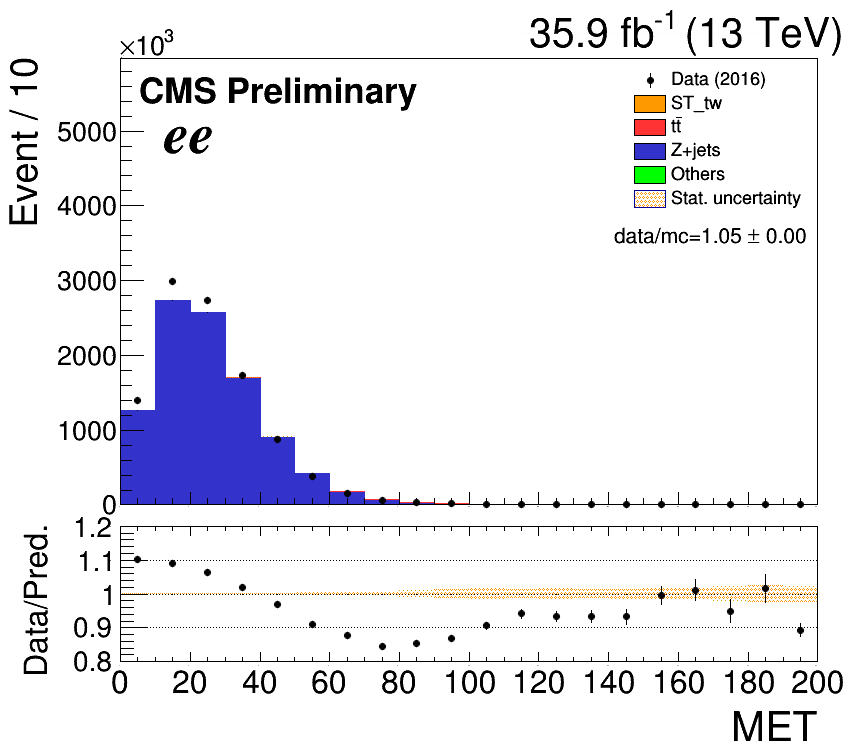
\includegraphics[width=0.45\textwidth]{figures/tW/fig/Step1/ee_noNvtx/H_MET_Et.png}&
      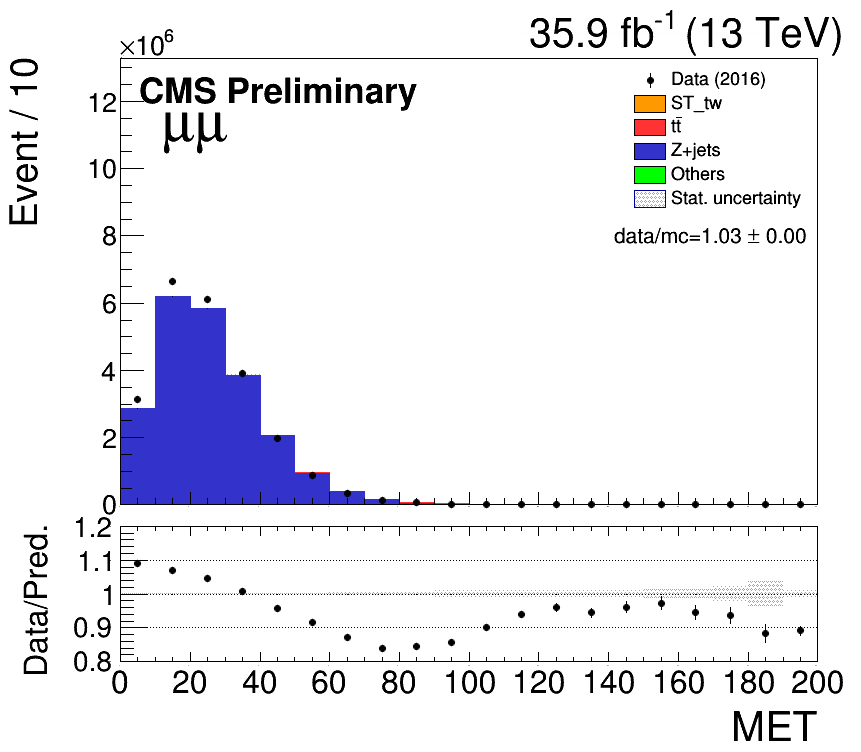
\includegraphics[width=0.45\textwidth]{figures/tW/fig/Step1/mumu_noNvtx/H_MET_Et.png}\\
    \end{tabular}
    \caption{The distributions of MET for $ee$ (left) and $\mu\mu$ (right) channels after step 1 selection. All backgrounds are estimated from MC.}
    \label{fig:step1_MET_phi}
  \end{center}
\end{figure}

%\begin{table}[h]
%\centering
%\begin{tabular}{|l|l|c|c|}
%\hline
%\multirow{3}{*}{Step 1}         &                                                       & $ee$ and $\mu\mu$     & $e\mu$        \\ \cline{2-4}
%                                & $p_{T}^{\text{leading lepton}}>$ 25 GeV and $p_{T}^{\text{sub-leading lepton}}>$ 20 GeV & $\surd$               & $\surd$       \\ \cline{2-4}
%                                & Mass(ll)$>$ 20 GeV                                    & $\surd$               & $\surd$       \\ \cline{2-4}
%                                & The two highest $p_{T}$ leptons should have opoosite charge       & $\surd$               & $\surd$       \\ \hline
%\multirow{2}{*}{Step 2}         & MET $>$ 60 GeV                                        & $\surd$               & -       \\ \cline{2-4}
%                                & Mass(ll) $<76$ or $>106$ GeV                          & $\surd$               & -            \\ \hline
%\end{tabular}
%\caption{Event Selections}
%\label{tab:Event-selection}
%\end{table}

%\begin{table}[ht]
%\centering
%\begin{tabular}{|c|c|c||c|c|}
%\hline
%Channel & $ee$                   & fraction & $\mu\mu$            &fraction \\ \hline
%tW      & 8242      +/- 26       & 0.08\%   & 16259     +/- 37    & 0.07\%  \\ \hline
%TTbar   & 82120     +/- 62       & 0.83\%   & 165203    +/- 90    & 0.73\%  \\ \hline
%DY      & 9822251   +/- 6708     & 98.82\%  & 22325807  +/- 10376 & 98.96\% \\ \hline
%WW      & 8774      +/- 47       & 0.09\%   & 18933     +/- 71    & 0.08\%  \\ \hline
%WG      & 1280      +/- 75       & 0.01\%   & 334       +/- 38    & 0.00\%  \\ \hline
%Wjets   & 2173      +/- 296      & 0.02\%   & 1910      +/- 283   & 0.01\%  \\ \hline
%WZ      & 11056     +/- 23       & 0.11\%   & 22753     +/- 33    & 0.10\%  \\ \hline
%TTG     & 434       +/- 10       & 0.00\%   & 761       +/- 13    & 0.00\%  \\ \hline
%ZZ      & 2712      +/- 3        & 0.03\%   & 5880      +/- 5     & 0.03\%  \\ \hline
%HWW     & 782       +/- 11       & 0.01\%   & 1885      +/- 18    & 0.01\%  \\ \hline
%TTWJets & 38        +/- 4        & 0.00\%   & 72        +/- 5     & 0.00\%  \\ \hline \hline
%data    & 10406970  +/- 3226     &          & 23278344  +/- 4825  &         \\ \hline
%Pred    & 9939863   +/- 6715     &          & 22559798  +/- 10381 &         \\ \hline
%
%\hline
%\hline
%Channel & $e\mu$          & fraction   & $Combined$          &fraction \\ \hline
%tW      & 23057   +/- 43  & 6.43\%     & 47558     +/- 62    & 0.14\%  \\ \hline
%TTbar   & 232161  +/- 106 & 64.76\%    & 479484    +/- 153   & 1.46\%  \\ \hline
%DY      & 64880   +/- 559 & 18.10\%    & 32212938  +/- 12368 & 98.04\% \\ \hline
%WW      & 25864   +/- 82  & 7.21\%     & 53571     +/- 118   & 0.16\%  \\ \hline
%WG      & 1958    +/- 95  & 0.55\%     & 3572      +/- 127   & 0.01\%  \\ \hline
%Wjets   & 4060    +/- 412 & 1.13\%     & 8142      +/- 581   & 0.02\%  \\ \hline
%WZ      & 2369    +/- 14  & 0.66\%     & 36179     +/- 43    & 0.11\%  \\ \hline
%TTG     & 1115    +/- 16  & 0.31\%     & 2310      +/- 23    & 0.01\%  \\ \hline
%ZZ      & 484     +/- 2   & 0.13\%     & 9076      +/- 7     & 0.03\%  \\ \hline
%HWW     & 2430    +/- 20  & 0.68\%     & 5097      +/- 29    & 0.02\%  \\ \hline
%TTWJets & 121     +/- 7   & 0.03\%     & 231       +/- 9     & 0.00\%  \\ \hline \hline
%data    & 356383  +/- 597 &            & 34041697  +/- 5835  &         \\ \hline
%Pred    & 358497  +/- 716 &            & 32858157  +/- 12384 &         \\ \hline
%
%\end{tabular}
%\caption{Cut flow Table after step1 (trigger and lepton selections). Number of background events  are estimated using MC simulated samples and  errors are MC statistical uncertainties only. }
%\label{tab:cut_flow_step1}
%\end{table}
%
%\begin{figure}[ht]
%  \begin{center}
%    \begin{tabular}{ccc}
%      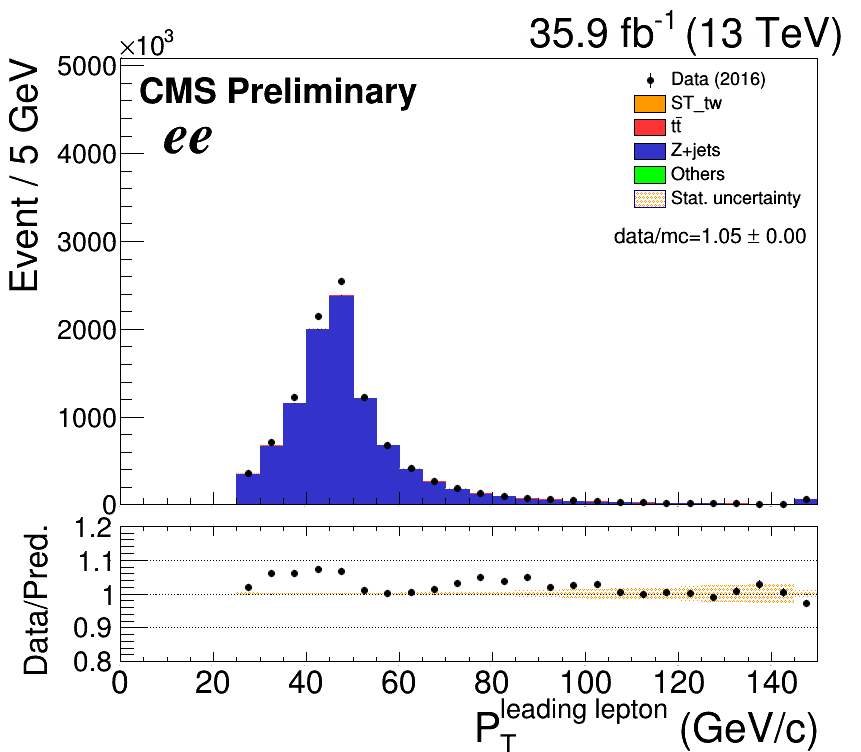
\includegraphics[width=0.32\textwidth]{figures/tW/fig/Step1/ee_noNvtx/H_lepton_led_pt.png}&
%      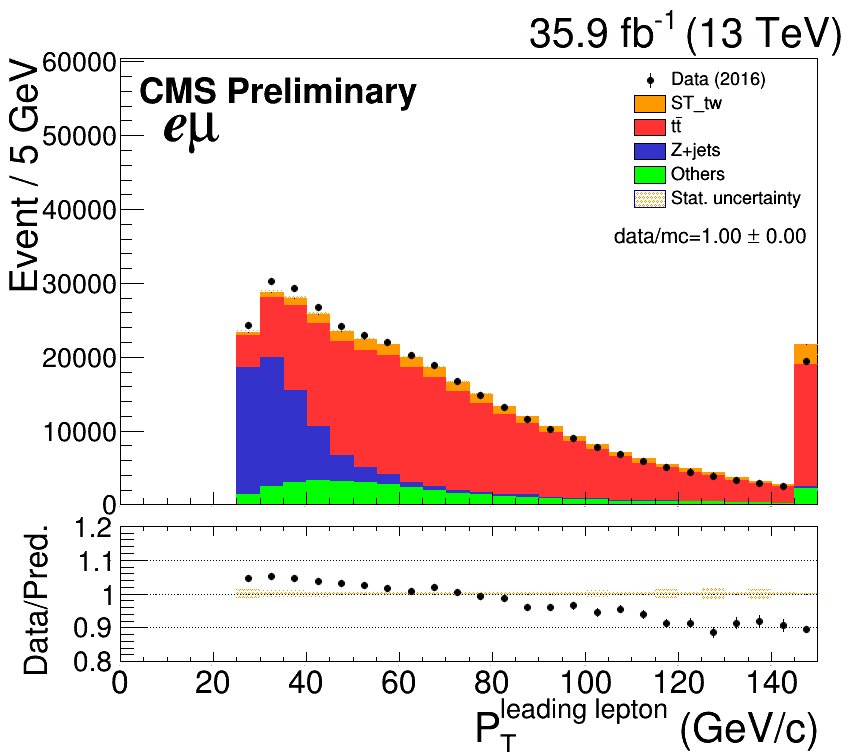
\includegraphics[width=0.32\textwidth]{figures/tW/fig/Step1/emu_noNvtx/H_lepton_led_pt.png}&
%      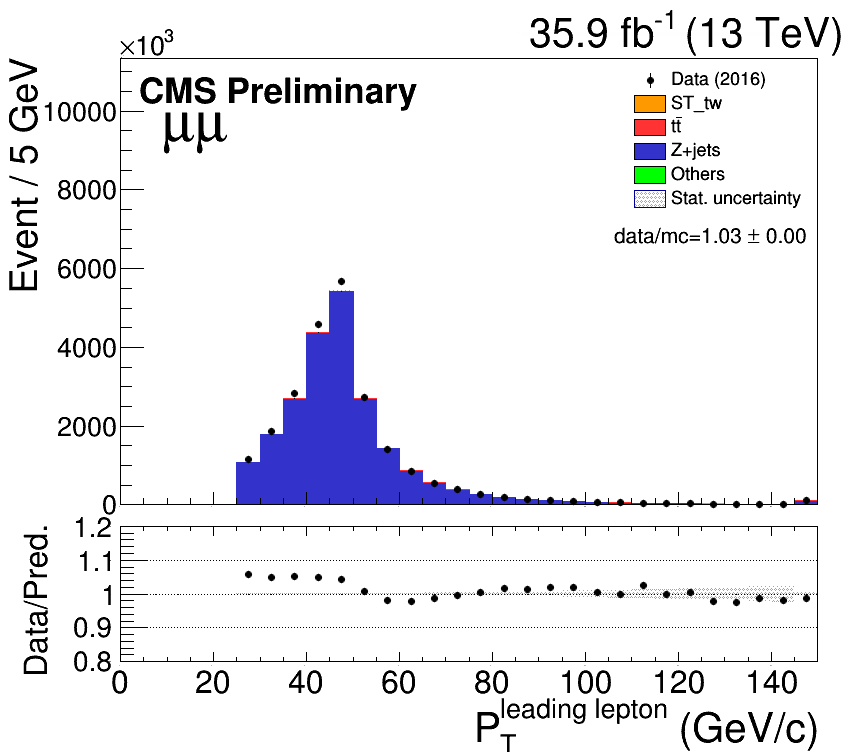
\includegraphics[width=0.32\textwidth]{figures/tW/fig/Step1/mumu_noNvtx/H_lepton_led_pt.png}\\
%      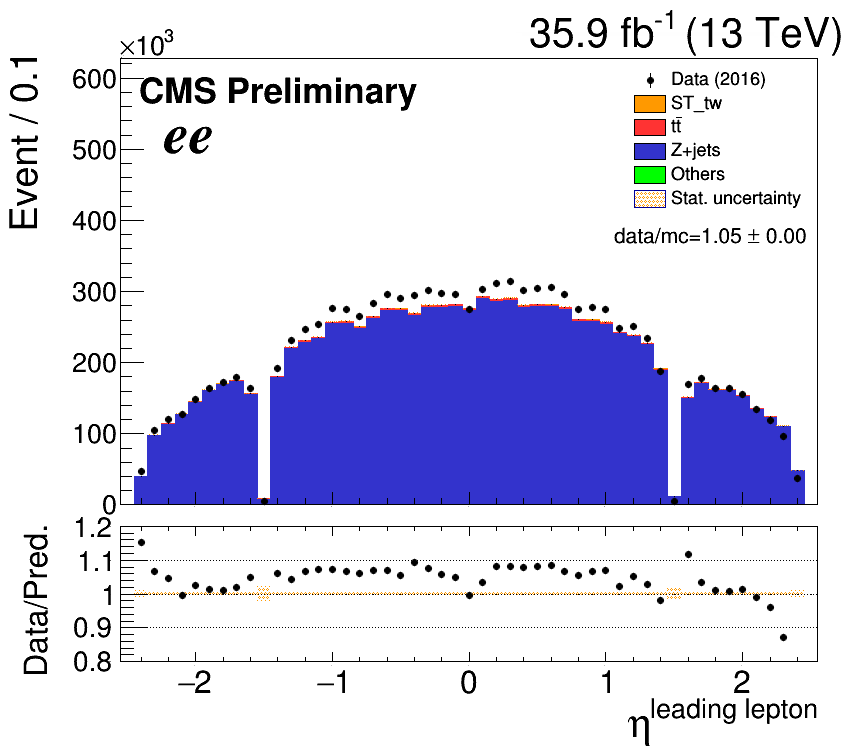
\includegraphics[width=0.32\textwidth]{figures/tW/fig/Step1/ee_noNvtx/H_lepton_led_eta.png}&
%      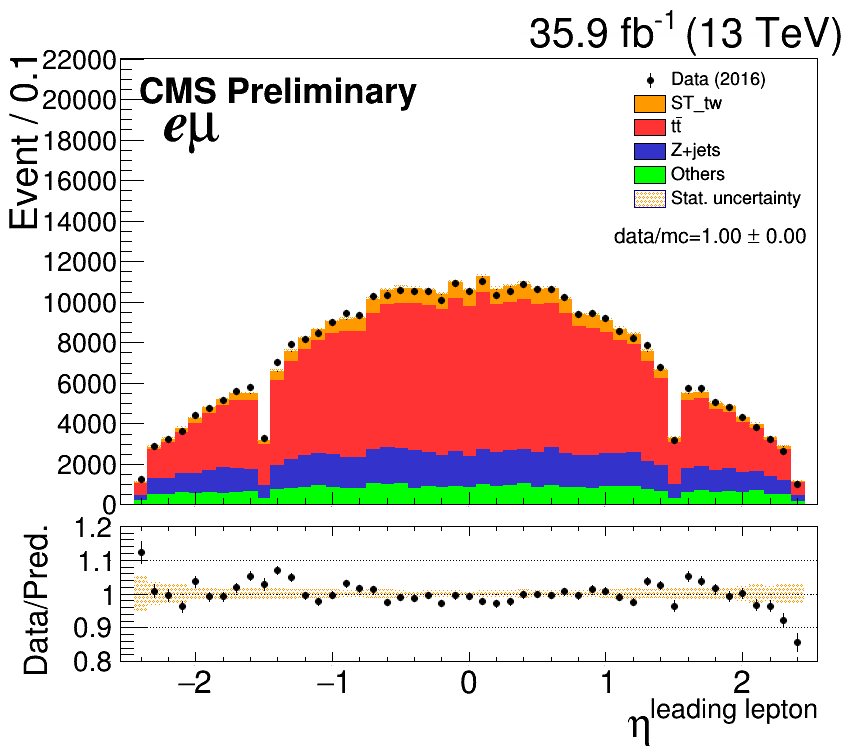
\includegraphics[width=0.32\textwidth]{figures/tW/fig/Step1/emu_noNvtx/H_lepton_led_eta.png}&
%      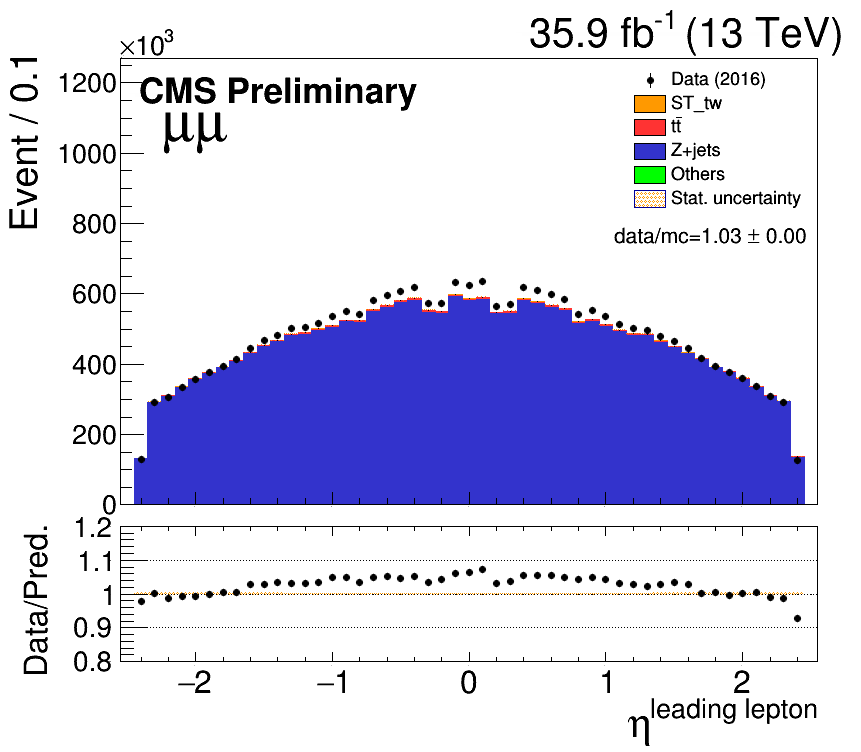
\includegraphics[width=0.32\textwidth]{figures/tW/fig/Step1/mumu_noNvtx/H_lepton_led_eta.png}\\
%      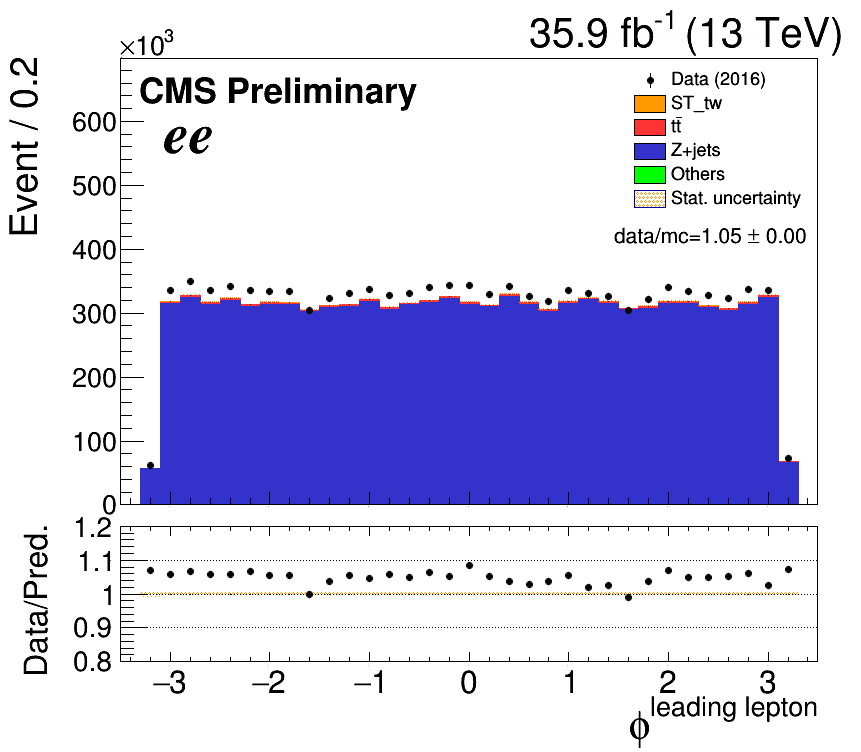
\includegraphics[width=0.32\textwidth]{figures/tW/fig/Step1/ee_noNvtx/H_lepton_led_phi.png}&
%      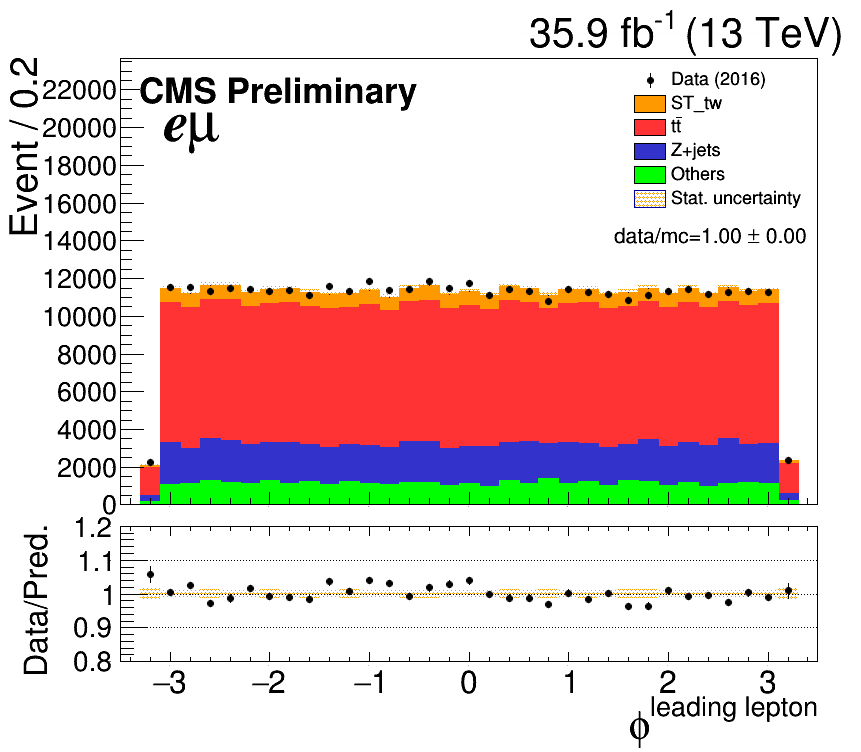
\includegraphics[width=0.32\textwidth]{figures/tW/fig/Step1/emu_noNvtx/H_lepton_led_phi.png}&
%      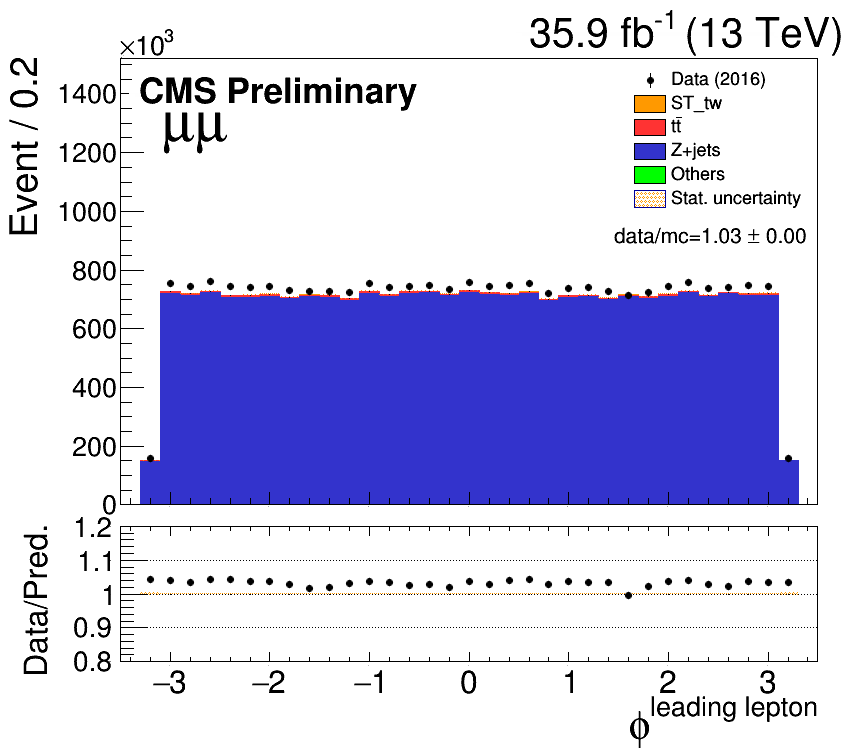
\includegraphics[width=0.32\textwidth]{figures/tW/fig/Step1/mumu_noNvtx/H_lepton_led_phi.png}\\
%    \end{tabular}
%    \caption{The distributions of Pt (top), $\eta$ (middle) and $\phi$ (bottom) of leading lepton for $ee$ (left), $e\mu$ (middle) and $\mu\mu$ (right) channels after step 1 (trigger and lepton selections). All backgrounds are estimated from MC.}
%    \label{fig:step1_leading_lepton1}
%  \end{center}
%\end{figure}
%
%\begin{figure}[ht]
%  \begin{center}
%    \begin{tabular}{ccc}
%      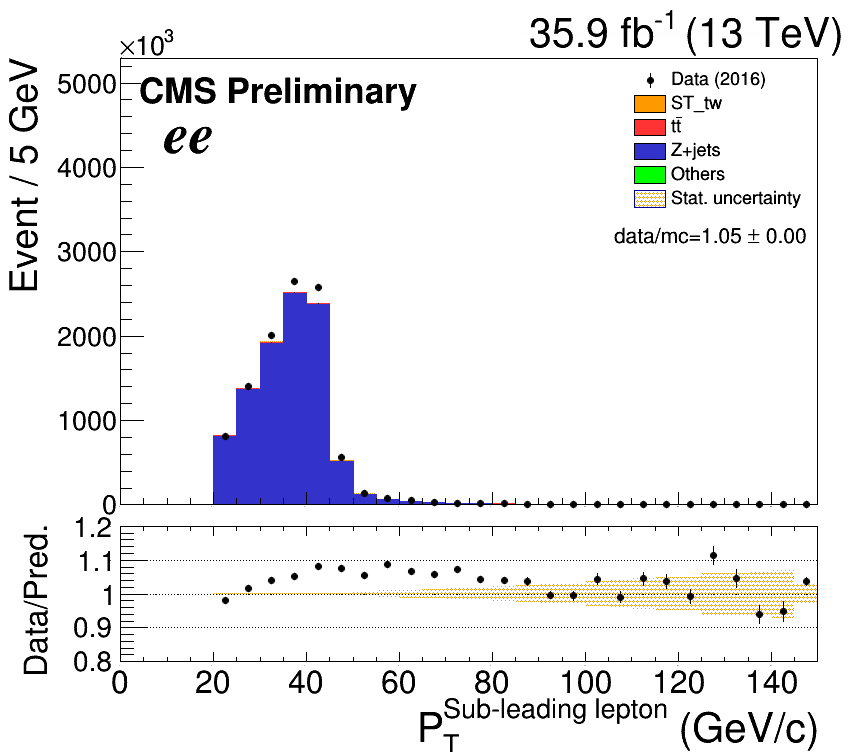
\includegraphics[width=0.32\textwidth]{figures/tW/fig/Step1/ee_noNvtx/H_lepton_sub_pt.png}&
%      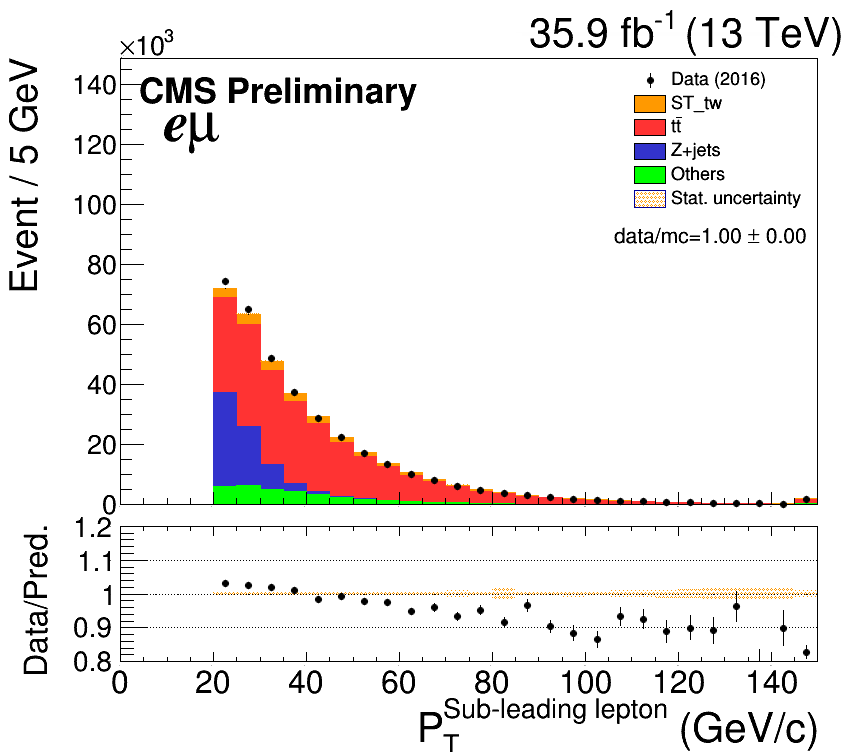
\includegraphics[width=0.32\textwidth]{figures/tW/fig/Step1/emu_noNvtx/H_lepton_sub_pt.png}&
%      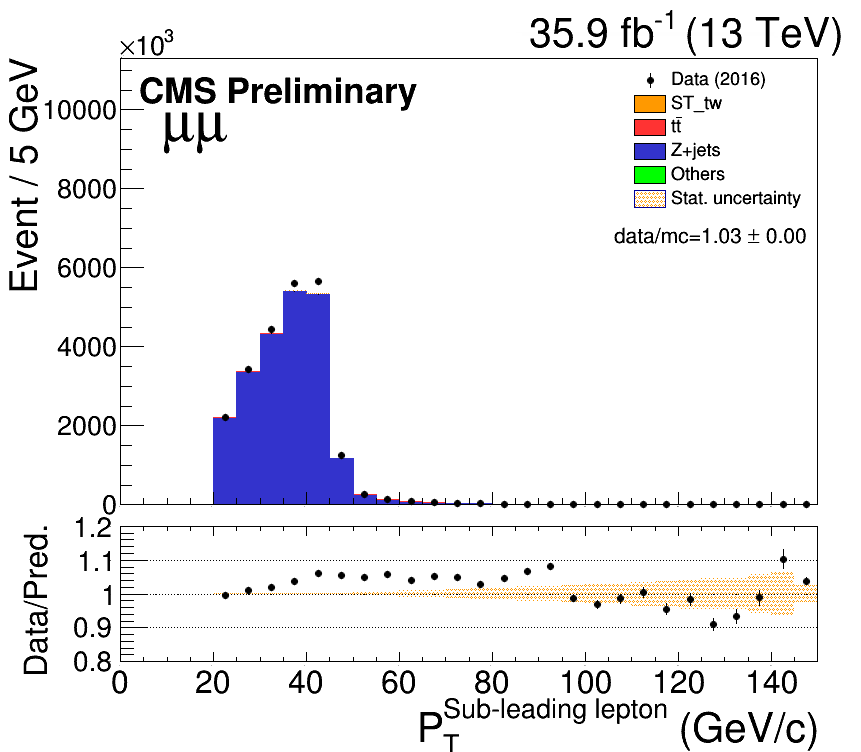
\includegraphics[width=0.32\textwidth]{figures/tW/fig/Step1/mumu_noNvtx/H_lepton_sub_pt.png}\\
%      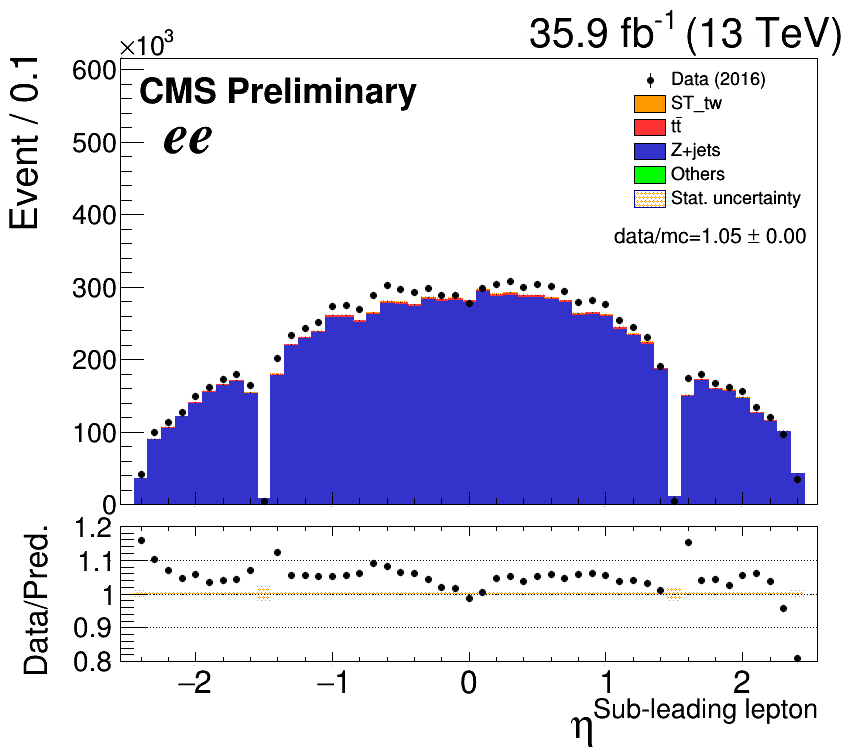
\includegraphics[width=0.32\textwidth]{figures/tW/fig/Step1/ee_noNvtx/H_lepton_sub_eta.png}&
%      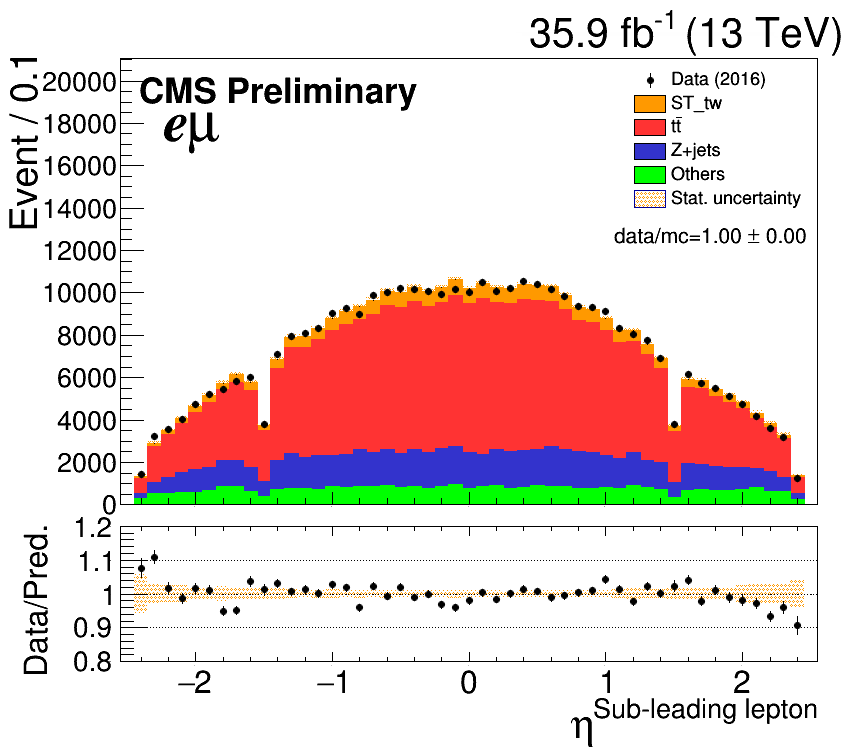
\includegraphics[width=0.32\textwidth]{figures/tW/fig/Step1/emu_noNvtx/H_lepton_sub_eta.png}&
%      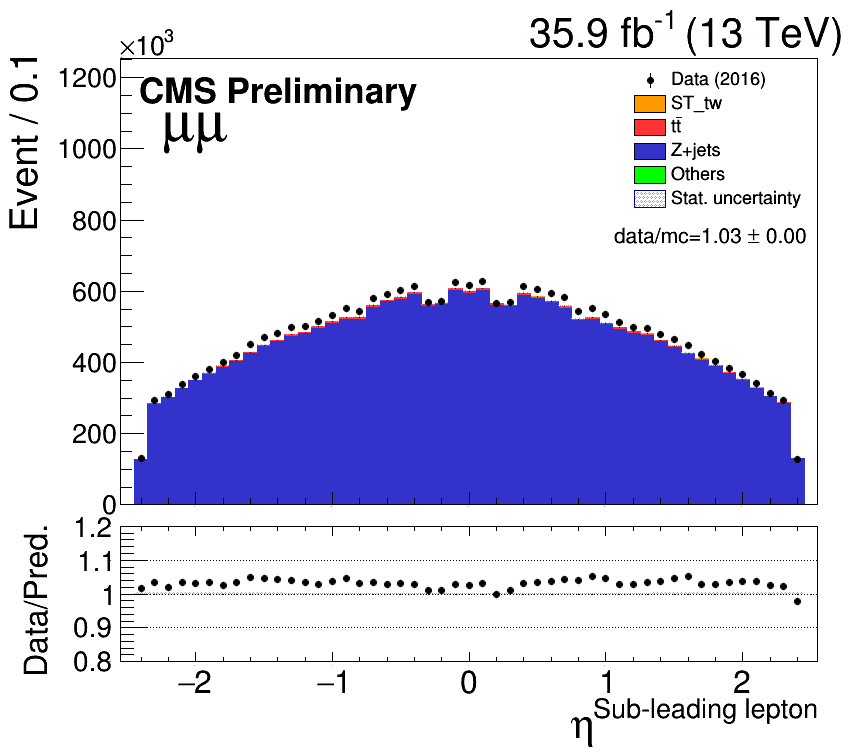
\includegraphics[width=0.32\textwidth]{figures/tW/fig/Step1/mumu_noNvtx/H_lepton_sub_eta.png}\\
%      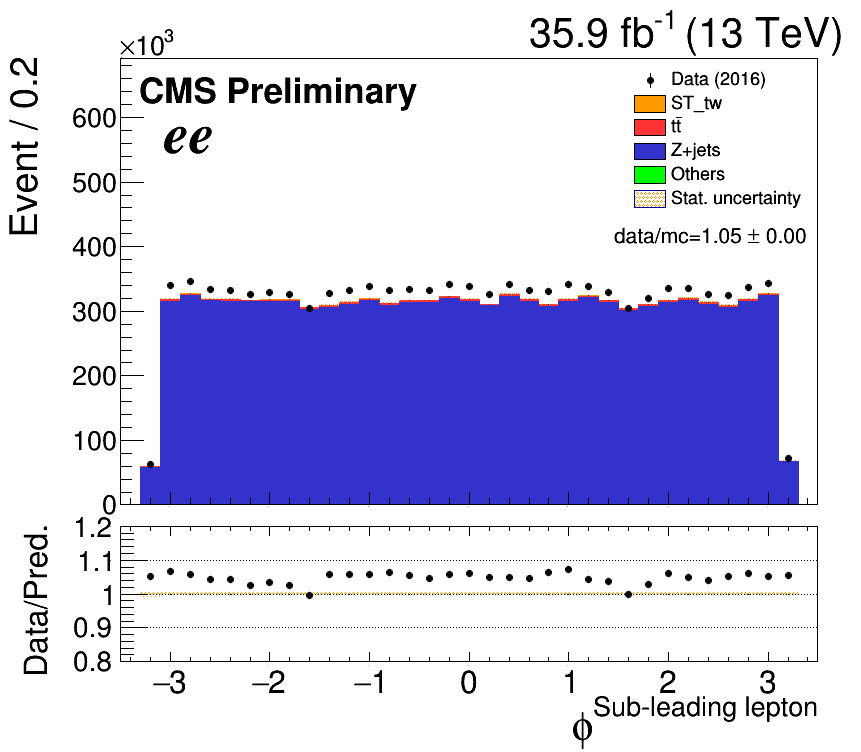
\includegraphics[width=0.32\textwidth]{figures/tW/fig/Step1/ee_noNvtx/H_lepton_sub_phi.png}&
%      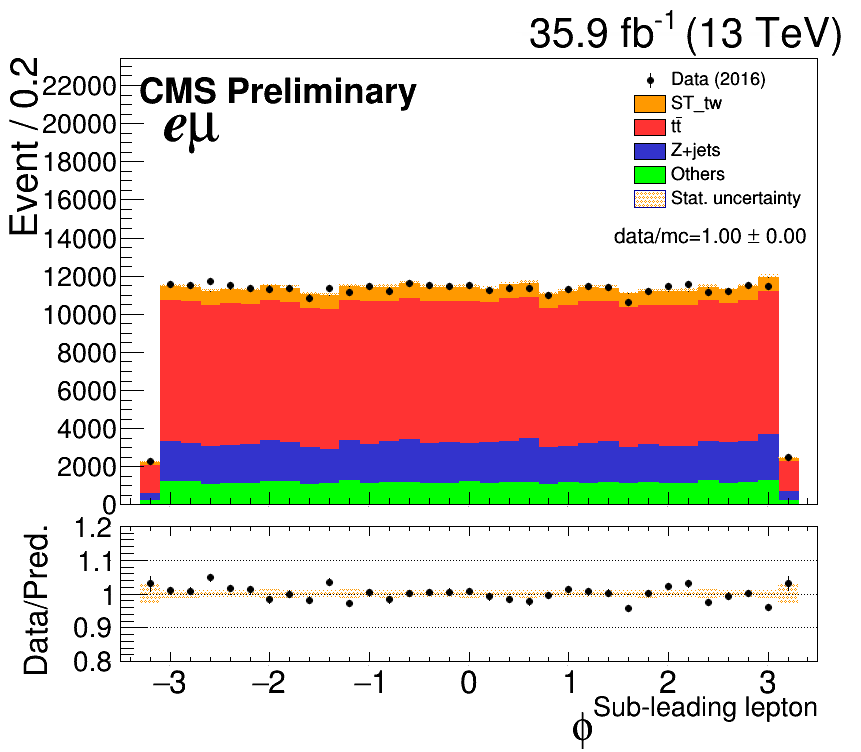
\includegraphics[width=0.32\textwidth]{figures/tW/fig/Step1/emu_noNvtx/H_lepton_sub_phi.png}&
%      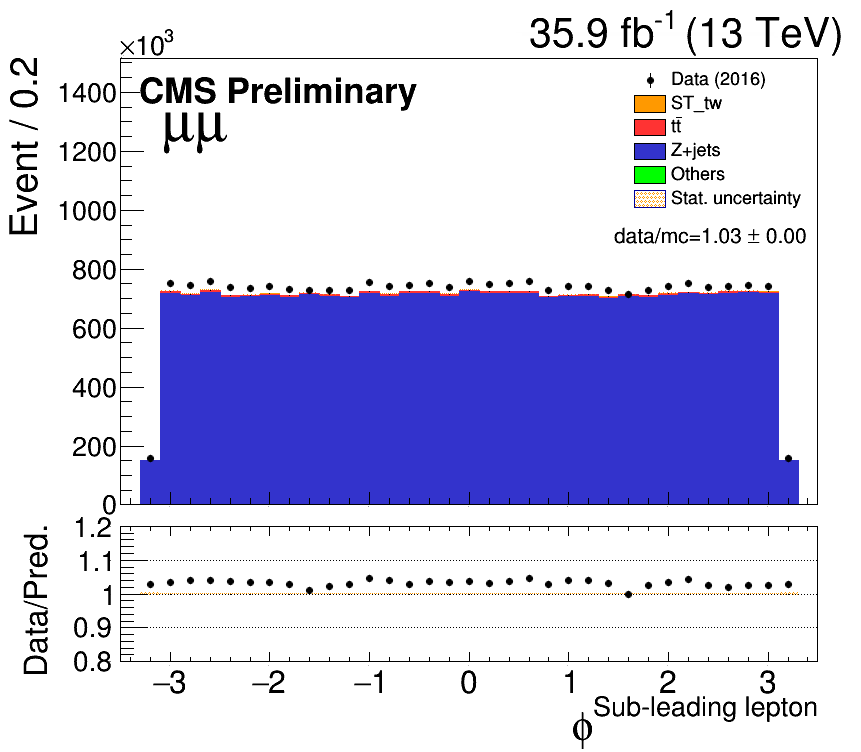
\includegraphics[width=0.32\textwidth]{figures/tW/fig/Step1/mumu_noNvtx/H_lepton_sub_phi.png}\\
%    \end{tabular}
%    \caption{The distributions of Pt (top), $\eta$ (middle) and $\phi$ (bottom) of sub-leading lepton for $ee$ (left), $e\mu$ (middle) and $\mu\mu$ (right) channels after step 1 (trigger and lepton selections). All backgrounds are estimated from MC.}
%    \label{fig:step1_leading_lepton}
%  \end{center}
%\end{figure}
%
%\begin{figure}[ht]
%  \begin{center}
%    \begin{tabular}{ccc}
%      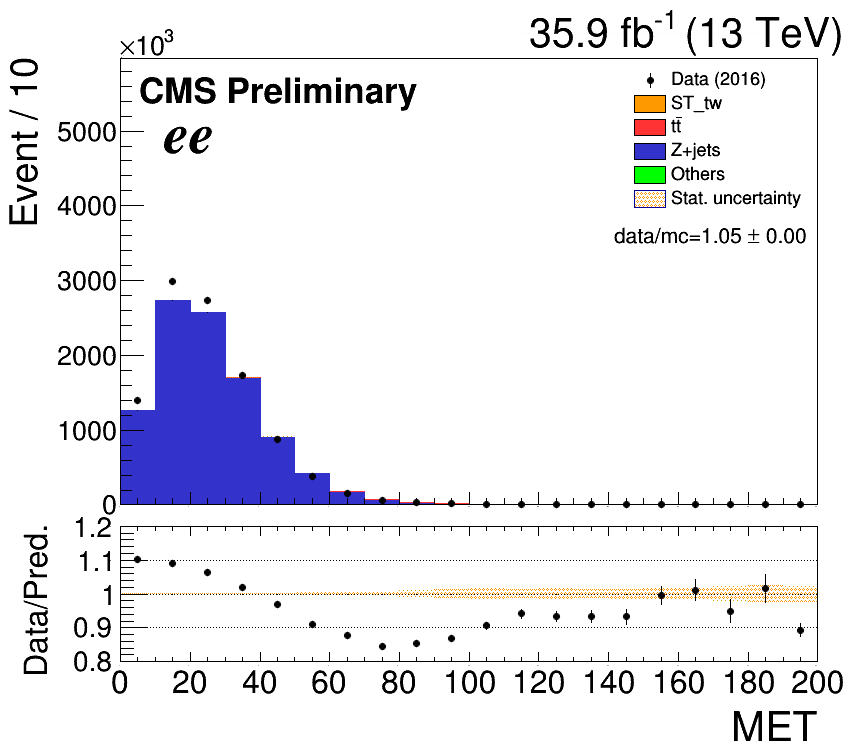
\includegraphics[width=0.32\textwidth]{figures/tW/fig/Step1/ee_noNvtx/H_MET_Et.png}&
%      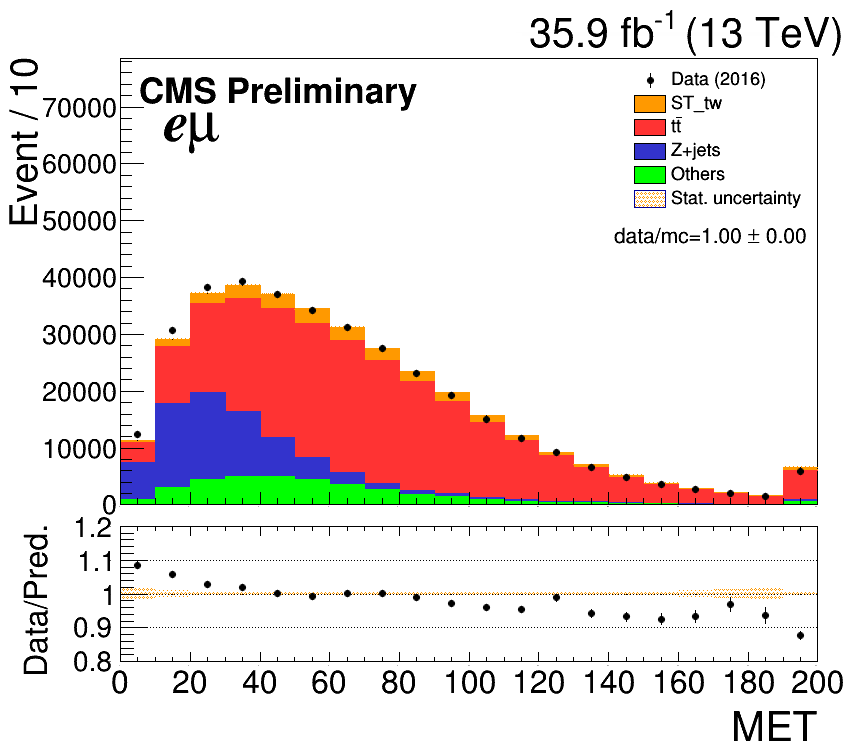
\includegraphics[width=0.32\textwidth]{figures/tW/fig/Step1/emu_noNvtx/H_MET_Et.png}&
%      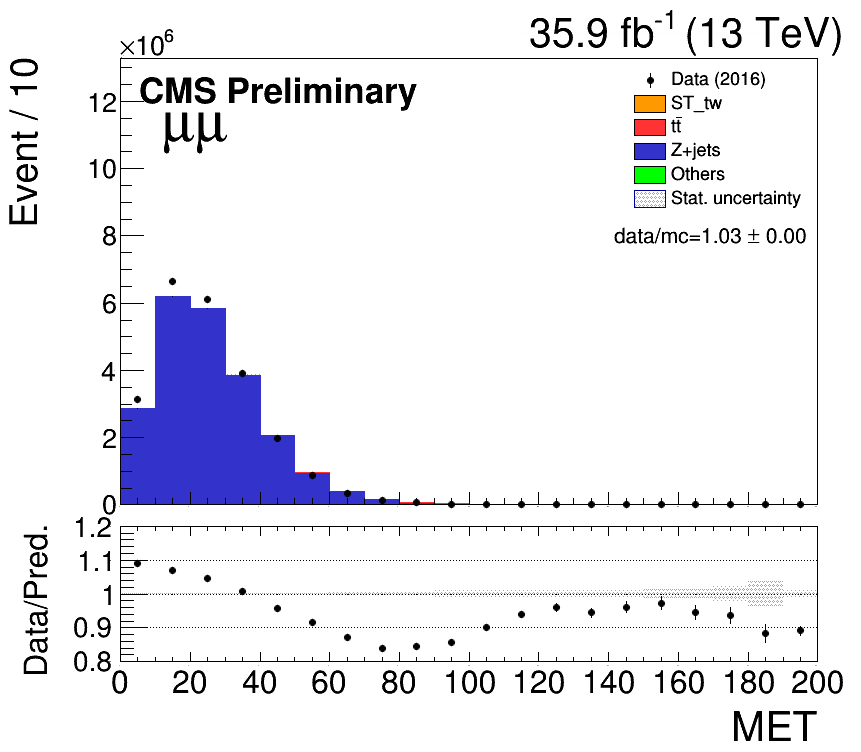
\includegraphics[width=0.32\textwidth]{figures/tW/fig/Step1/mumu_noNvtx/H_MET_Et.png}\\
%      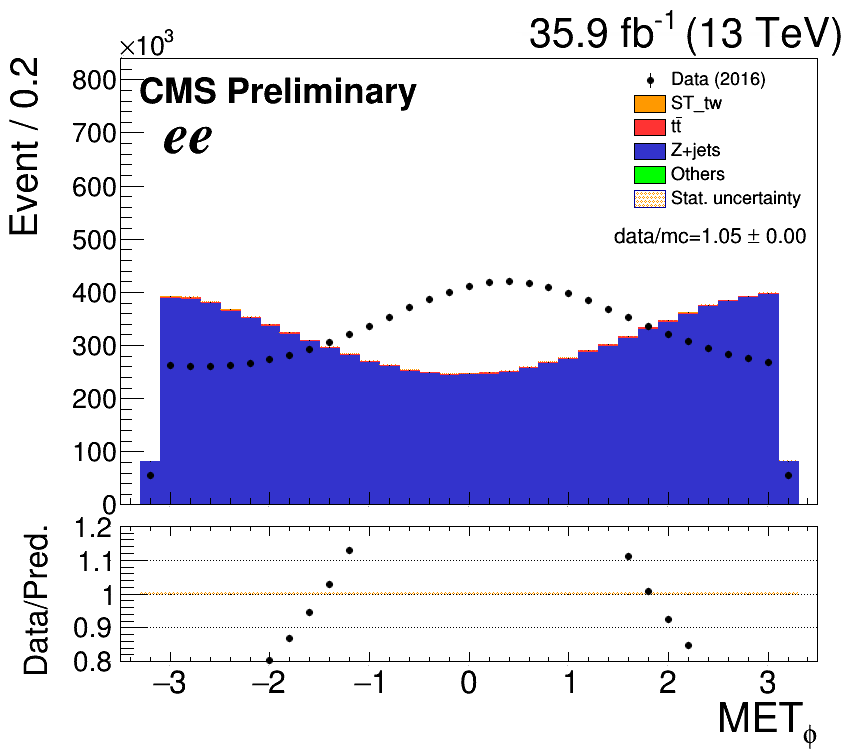
\includegraphics[width=0.32\textwidth]{figures/tW/fig/Step1/ee_noNvtx/H_MET_phi.png}&
%      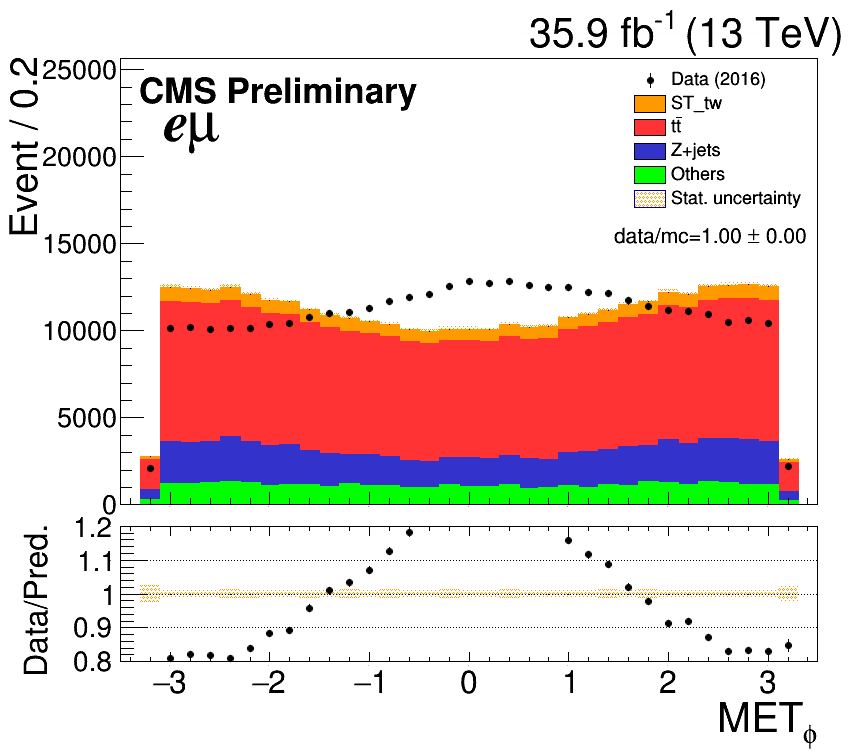
\includegraphics[width=0.32\textwidth]{figures/tW/fig/Step1/emu_noNvtx/H_MET_phi.png}&
%      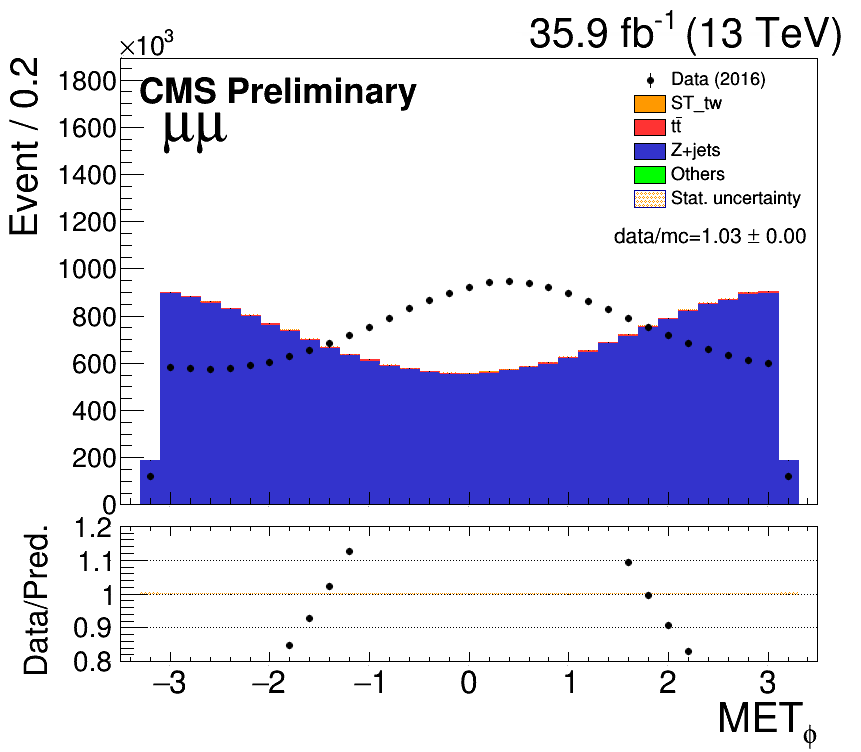
\includegraphics[width=0.32\textwidth]{figures/tW/fig/Step1/mumu_noNvtx/H_MET_phi.png}\\
%      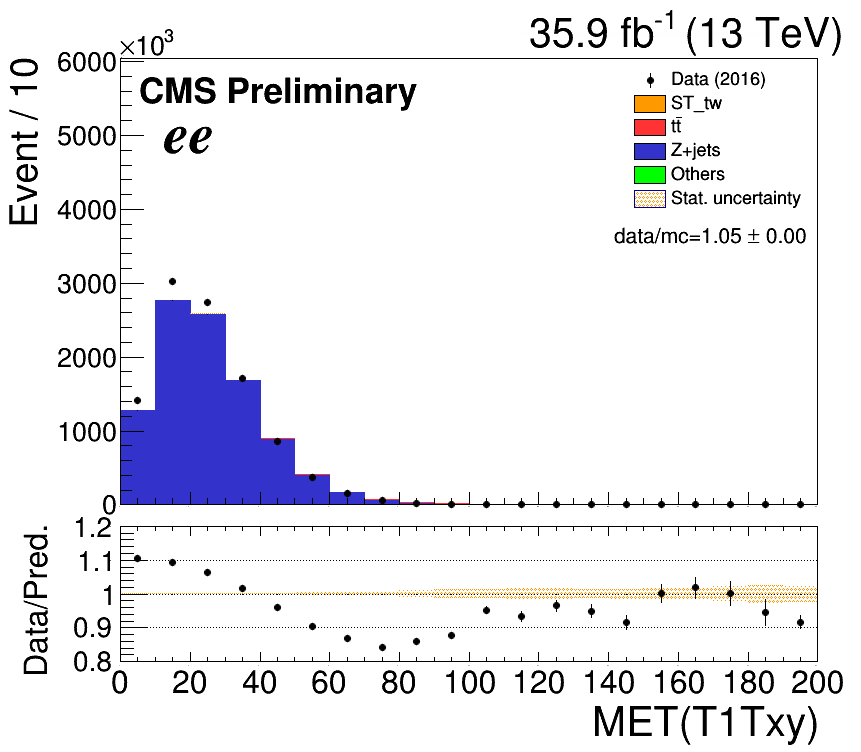
\includegraphics[width=0.32\textwidth]{figures/tW/fig/Step1/ee_noNvtx/H_MET_T1Txy_et.png}&
%      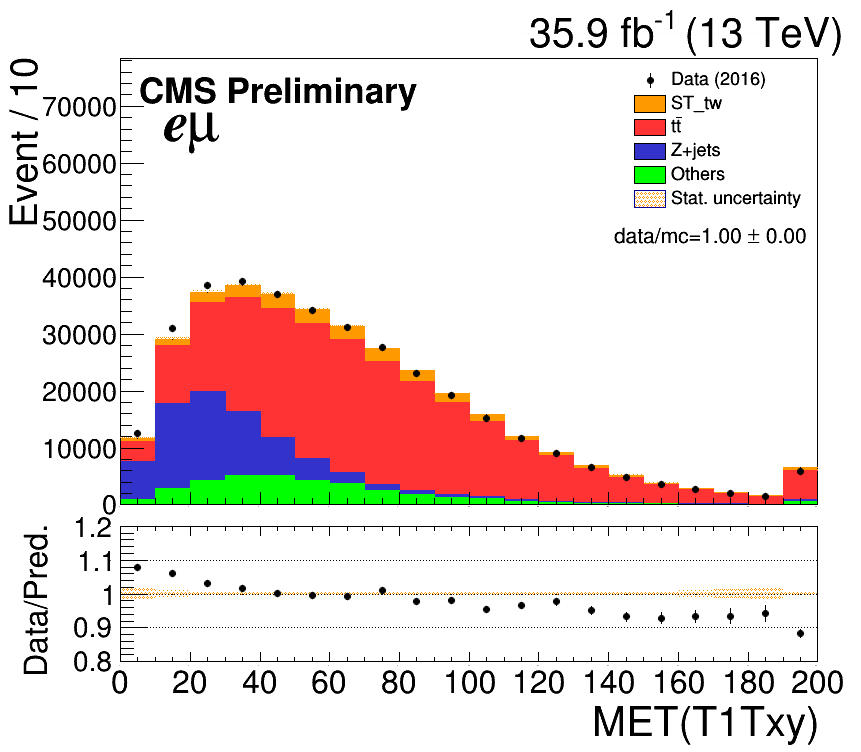
\includegraphics[width=0.32\textwidth]{figures/tW/fig/Step1/emu_noNvtx/H_MET_T1Txy_et.png}&
%      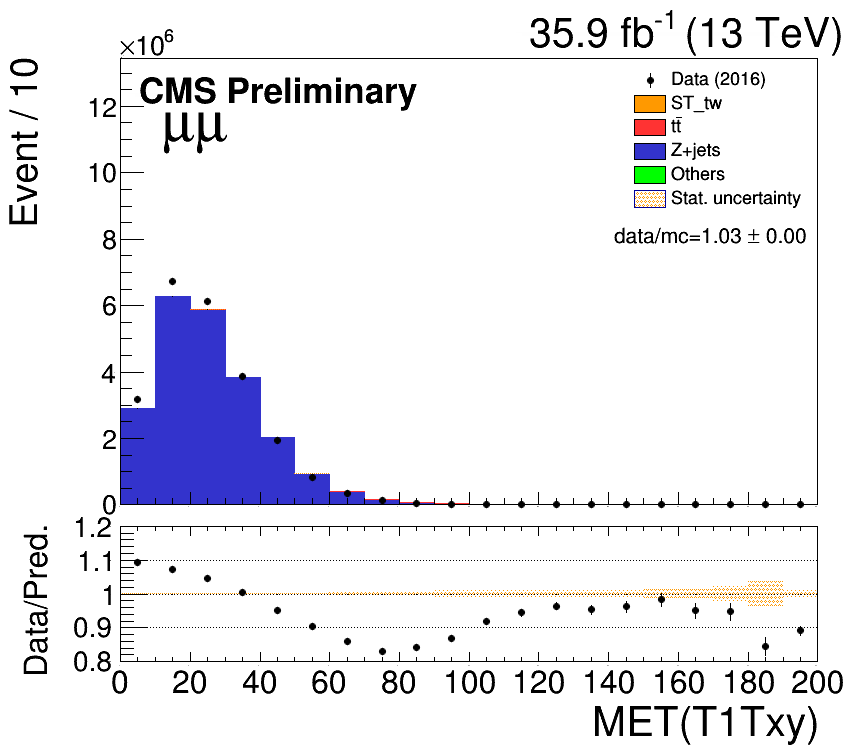
\includegraphics[width=0.32\textwidth]{figures/tW/fig/Step1/mumu_noNvtx/H_MET_T1Txy_et.png}\\
%      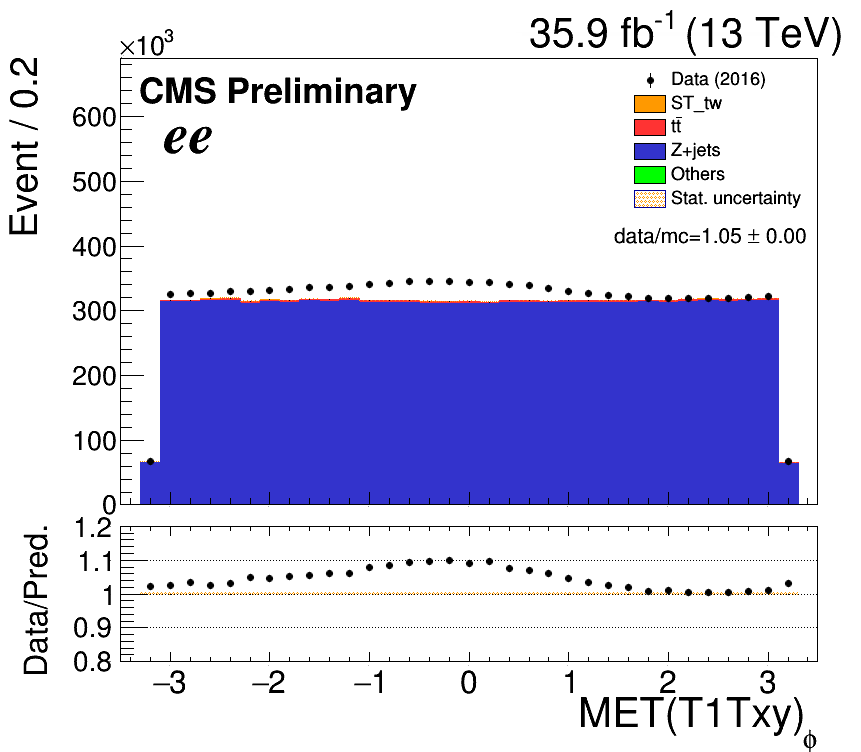
\includegraphics[width=0.32\textwidth]{figures/tW/fig/Step1/ee_noNvtx/H_MET_T1Txy_phi.png}&
%      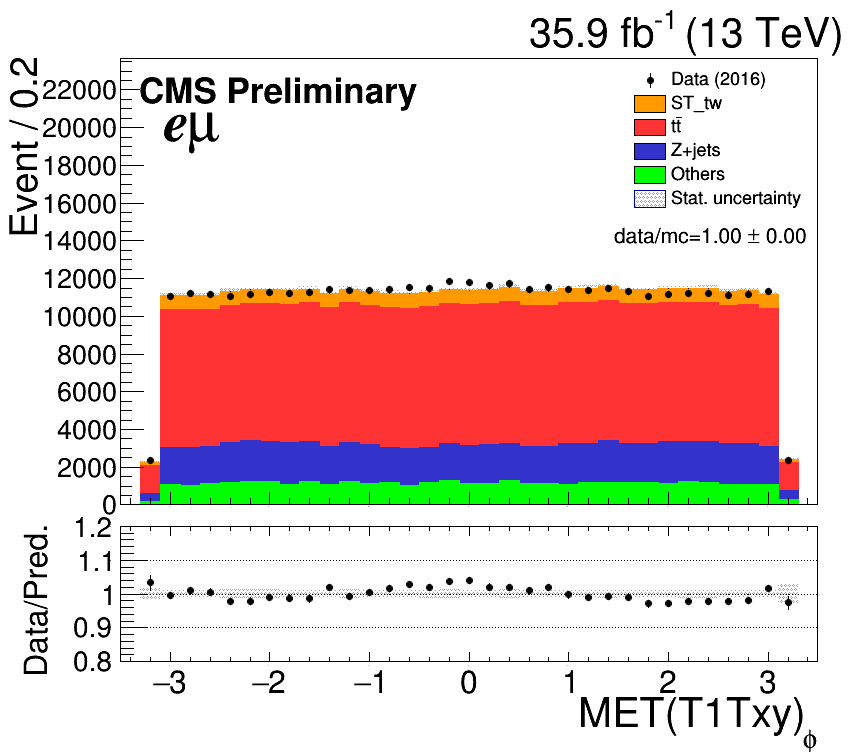
\includegraphics[width=0.32\textwidth]{figures/tW/fig/Step1/emu_noNvtx/H_MET_T1Txy_phi.png}&
%      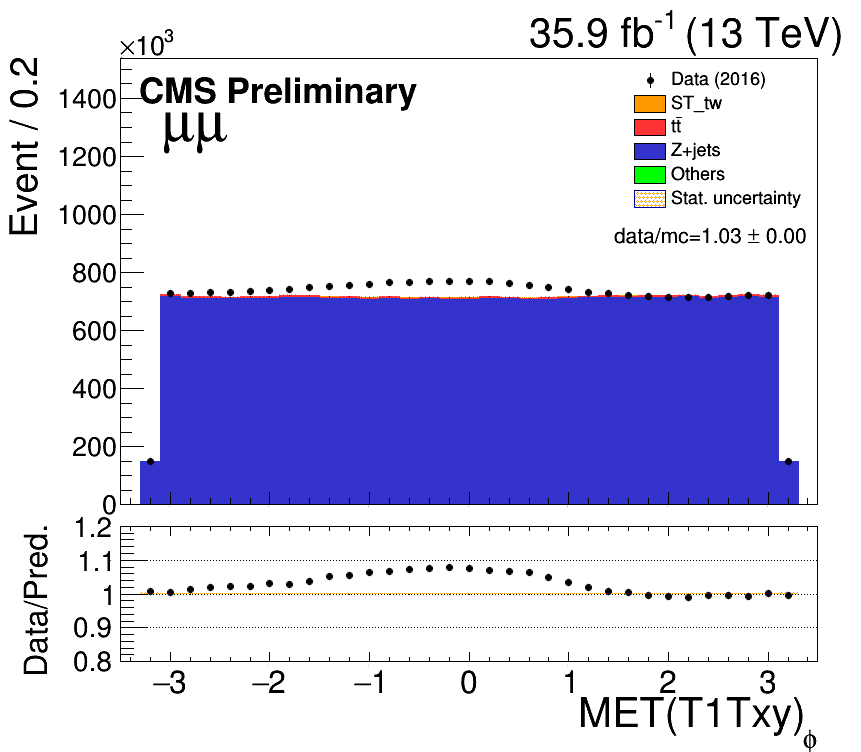
\includegraphics[width=0.32\textwidth]{figures/tW/fig/Step1/mumu_noNvtx/H_MET_T1Txy_phi.png}\\
%    \end{tabular}
%    \caption{The distributions of MET-T1 corrected (first row), $\phi$ of MET (second row), MET-T1-Txy corrected (third row) and $\phi$ of MET-T1-Txy corrected (last row) for $ee$ (left), $e\mu$ (middle) and $\mu\mu$ (right) channels after step 1 (trigger and lepton selections). All backgrounds are estimated from MC.}
%    \label{fig:step1_MET_phi}
%  \end{center}
%\end{figure}
%
%
%\begin{figure}[ht]
%  \begin{center}
%    \begin{tabular}{ccc}
%      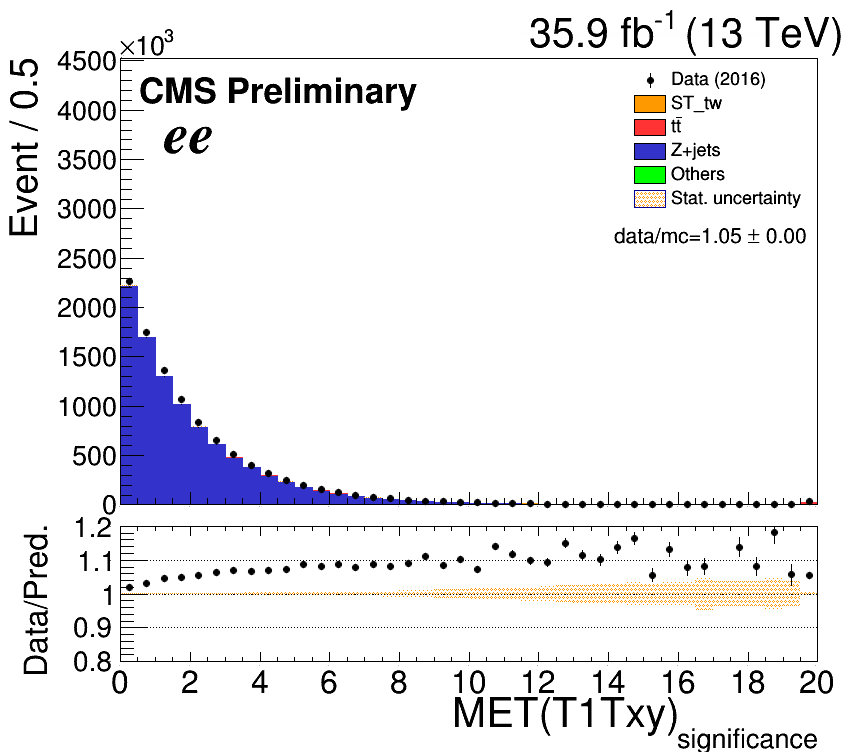
\includegraphics[width=0.32\textwidth]{figures/tW/fig/Step1/ee_noNvtx/H_MET_T1Txy_sf.png}&
%      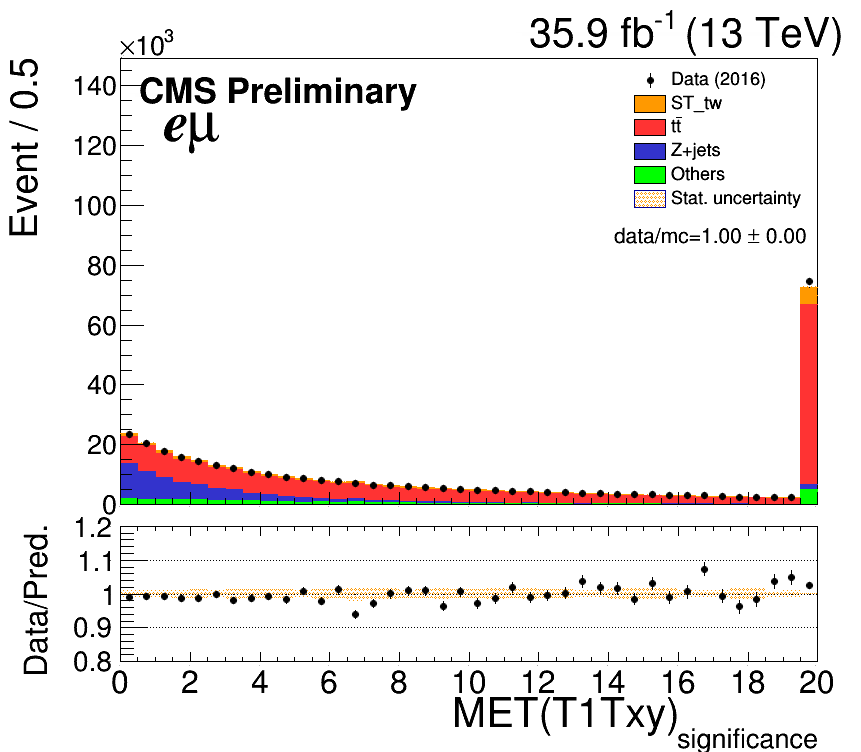
\includegraphics[width=0.32\textwidth]{figures/tW/fig/Step1/emu_noNvtx/H_MET_T1Txy_sf.png}&
%      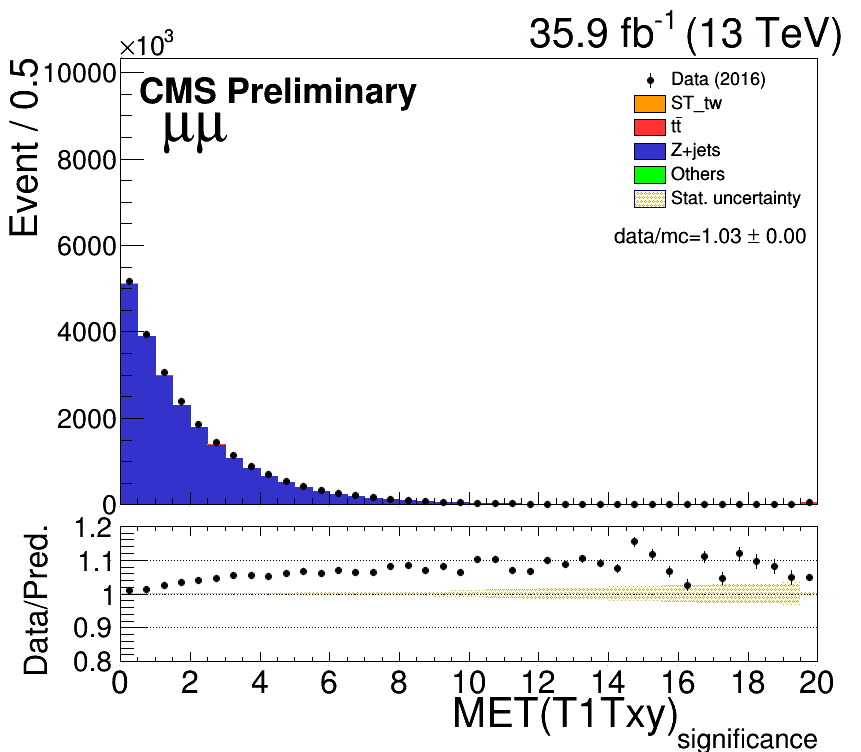
\includegraphics[width=0.32\textwidth]{figures/tW/fig/Step1/mumu_noNvtx/H_MET_T1Txy_sf.png}\\
%      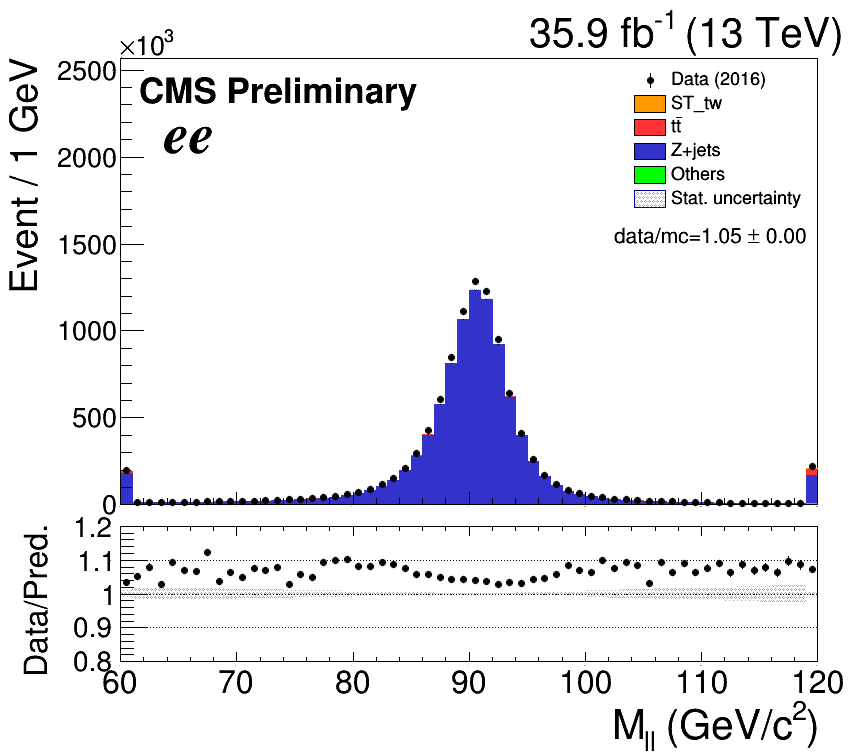
\includegraphics[width=0.32\textwidth]{figures/tW/fig/Step1/ee_noNvtx/H_Mll_Zpeak.png}&
%      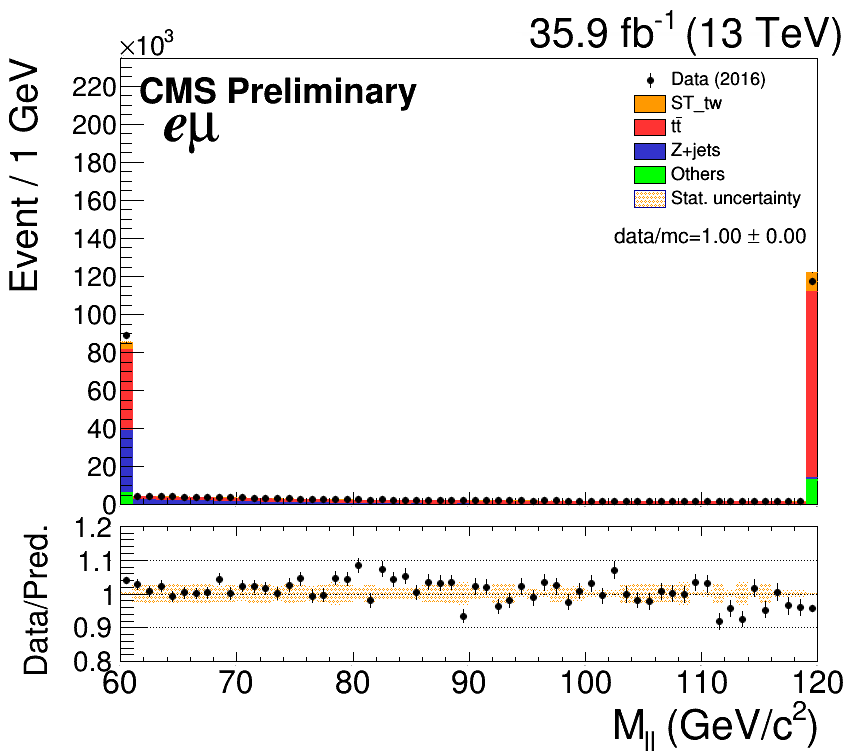
\includegraphics[width=0.32\textwidth]{figures/tW/fig/Step1/emu_noNvtx/H_Mll_Zpeak.png}&
%      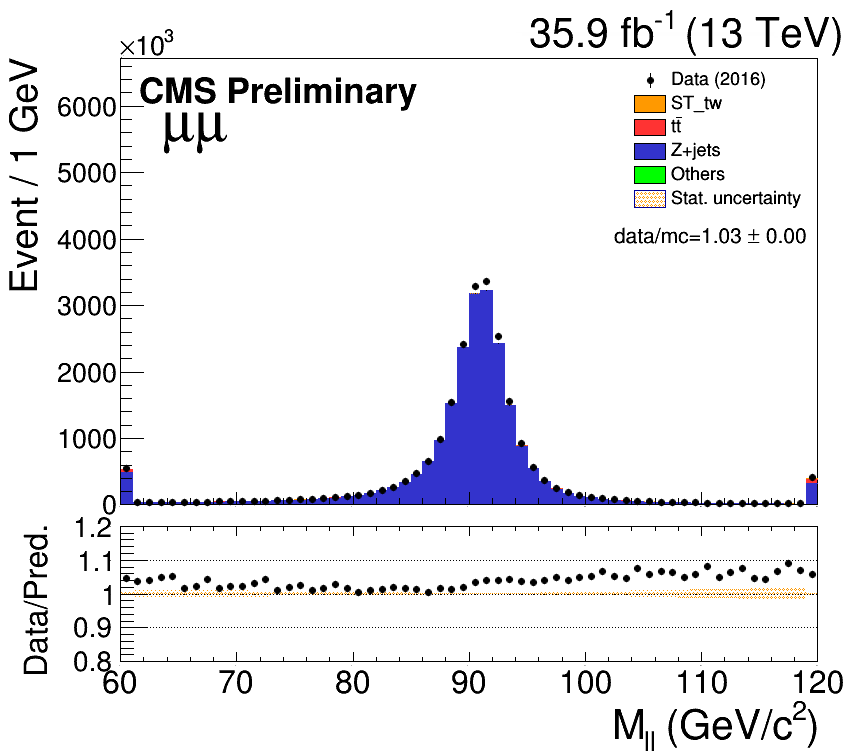
\includegraphics[width=0.32\textwidth]{figures/tW/fig/Step1/mumu_noNvtx/H_Mll_Zpeak.png}\\
%      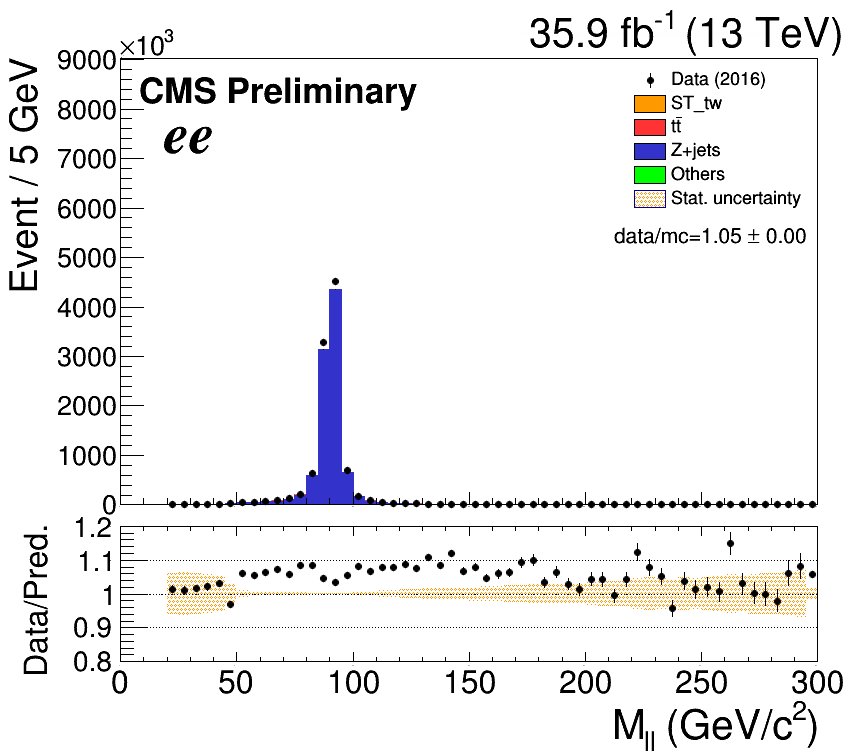
\includegraphics[width=0.32\textwidth]{figures/tW/fig/Step1/ee_noNvtx/H_Mll.png}&
%      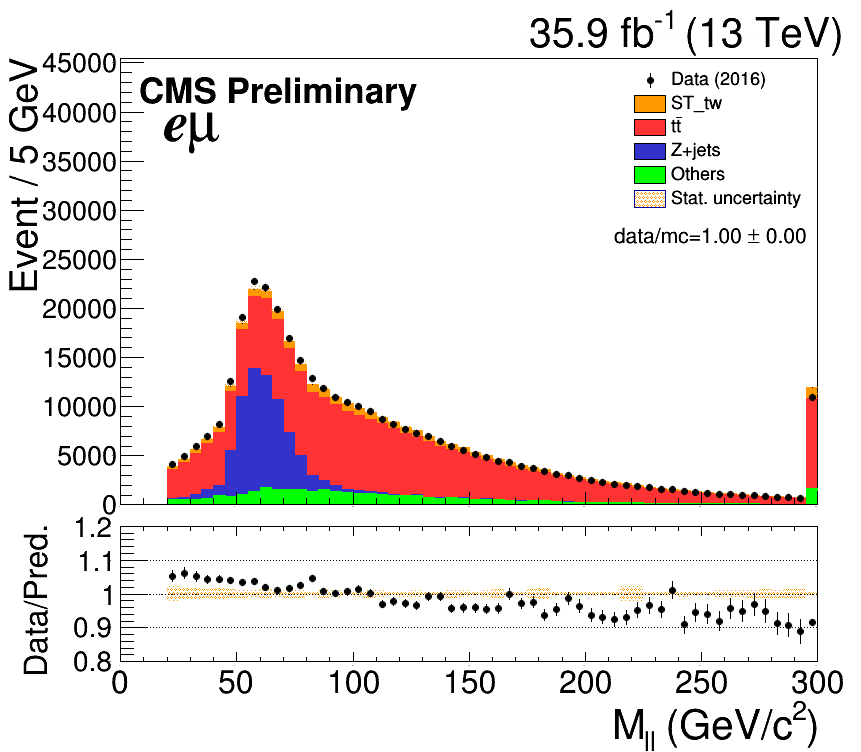
\includegraphics[width=0.32\textwidth]{figures/tW/fig/Step1/emu_noNvtx/H_Mll.png}&
%      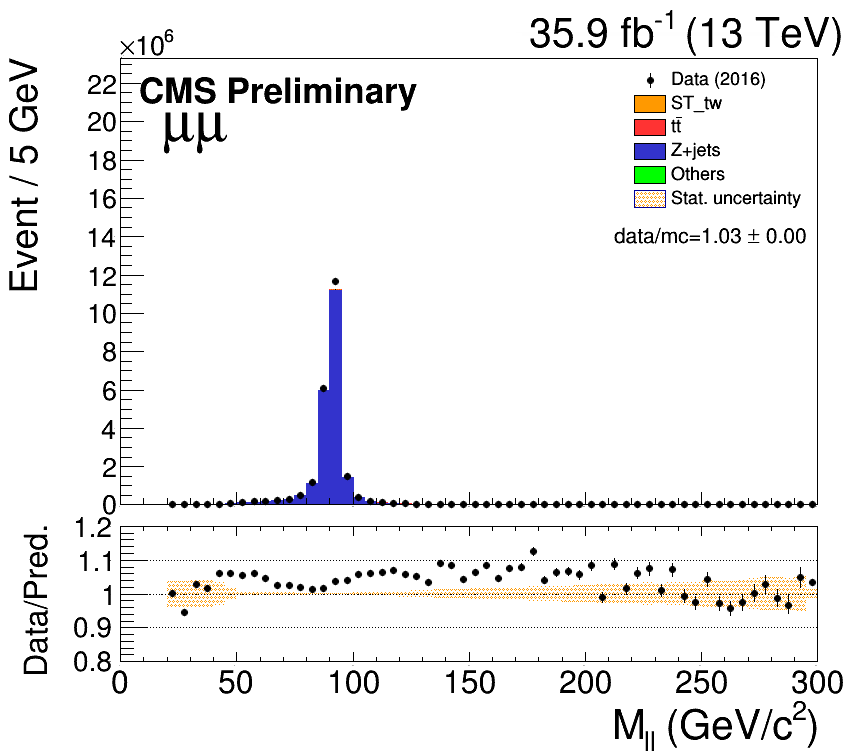
\includegraphics[width=0.32\textwidth]{figures/tW/fig/Step1/mumu_noNvtx/H_Mll.png}\\
%      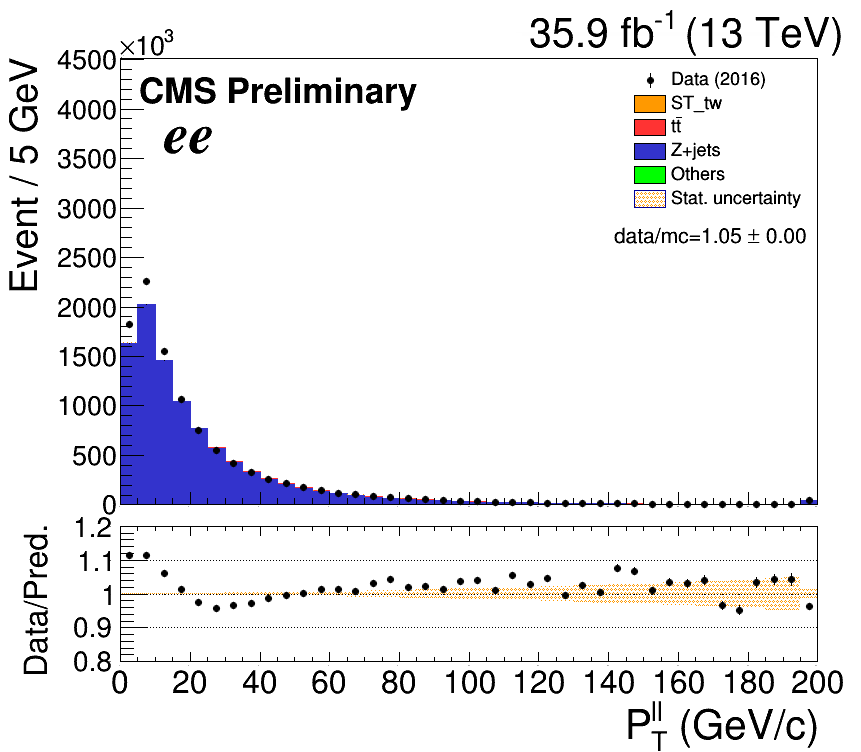
\includegraphics[width=0.32\textwidth]{figures/tW/fig/Step1/ee_noNvtx/H_Ptll.png}&
%      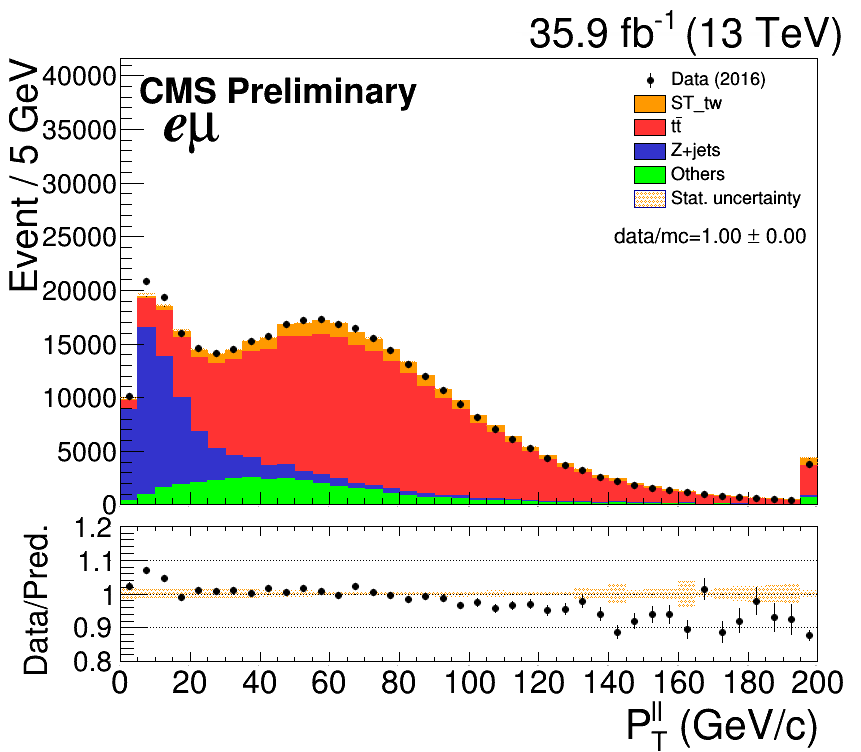
\includegraphics[width=0.32\textwidth]{figures/tW/fig/Step1/emu_noNvtx/H_Ptll.png}&
%      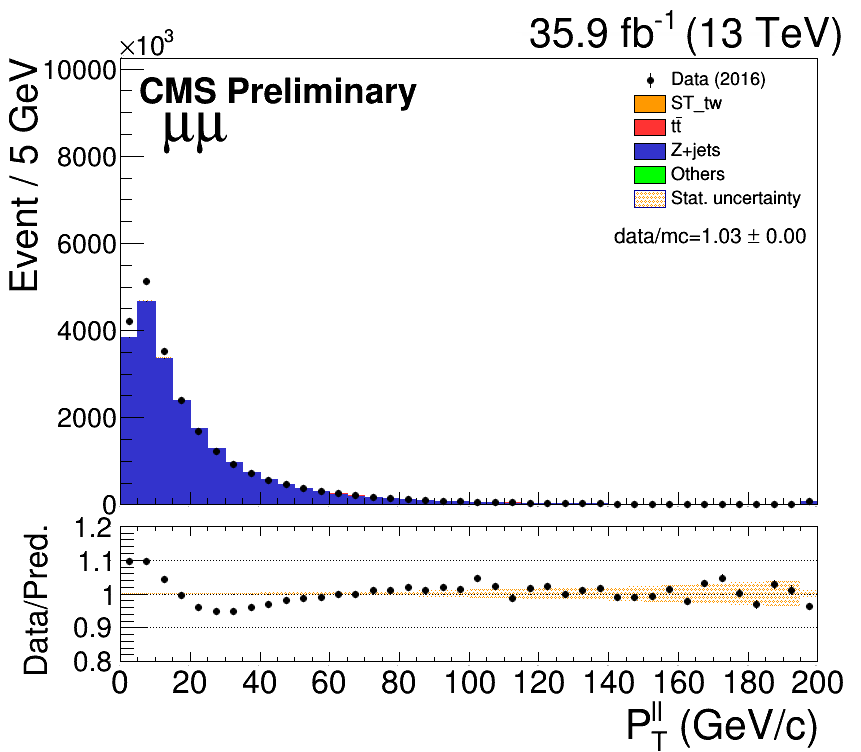
\includegraphics[width=0.32\textwidth]{figures/tW/fig/Step1/mumu_noNvtx/H_Ptll.png}\\
%    \end{tabular}
%    \caption{The distributions of MET significance (first row), invariant mass of two leptons in Z peak region [60-120] (second row), invariant mass of two leptons in wide range (third row) and Pt of two leptons system (last row) for $ee$ (left), $e\mu$ (middle) and $\mu\mu$ (right) channels after step 1 (trigger and lepton selections). All backgrounds are estimated from MC.}
%    \label{fig:step1_METsf_M_pt}
%  \end{center}
%\end{figure}
%
%\begin{figure}[ht]
%  \begin{center}
%    \begin{tabular}{ccc}
%      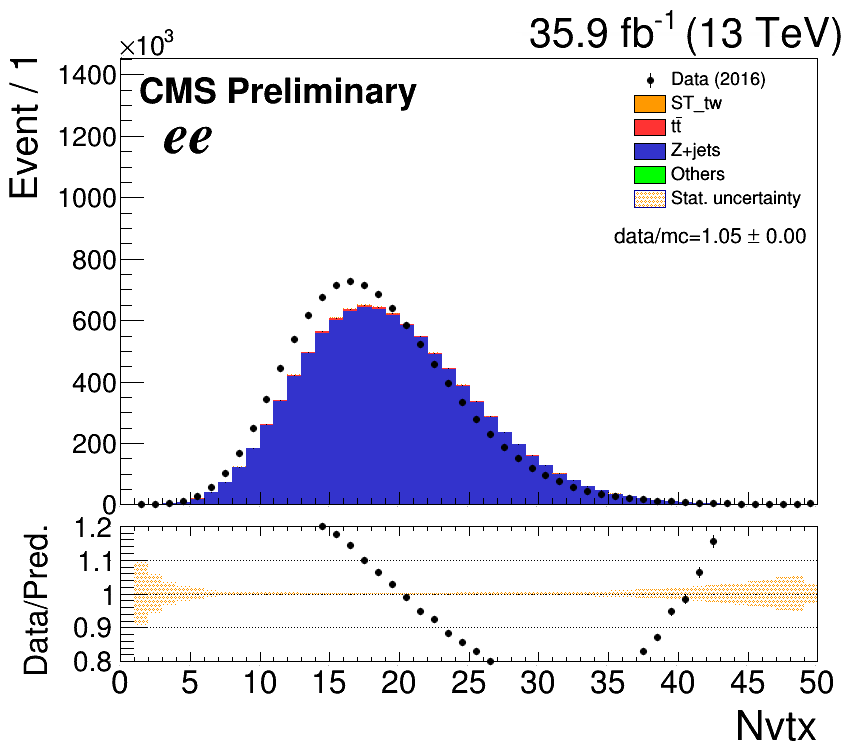
\includegraphics[width=0.32\textwidth]{figures/tW/fig/Step1/ee_noNvtx/H_pv_n.png}&
%      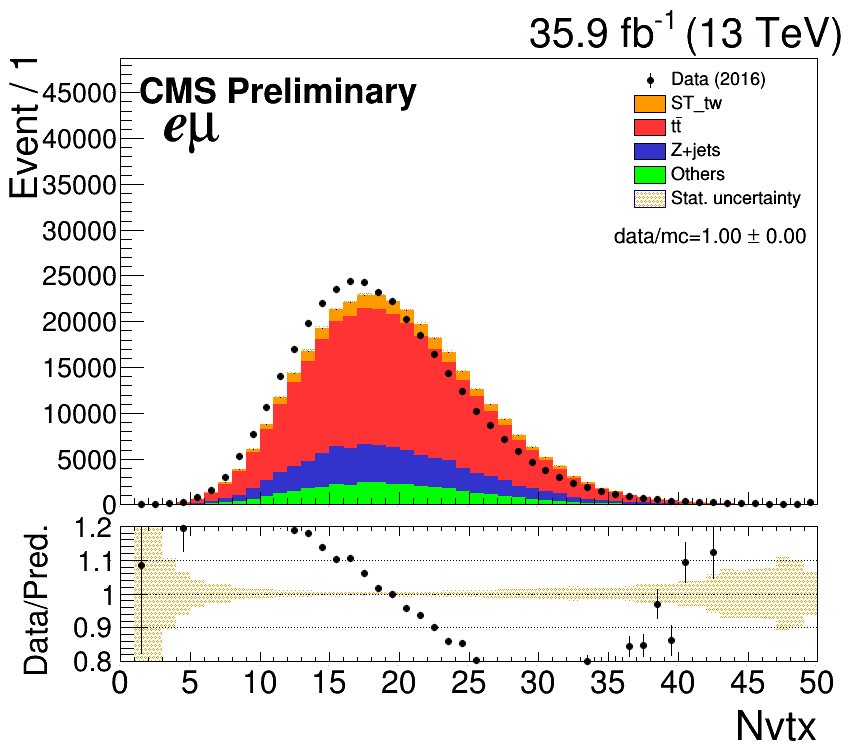
\includegraphics[width=0.32\textwidth]{figures/tW/fig/Step1/emu_noNvtx/H_pv_n.png}&
%      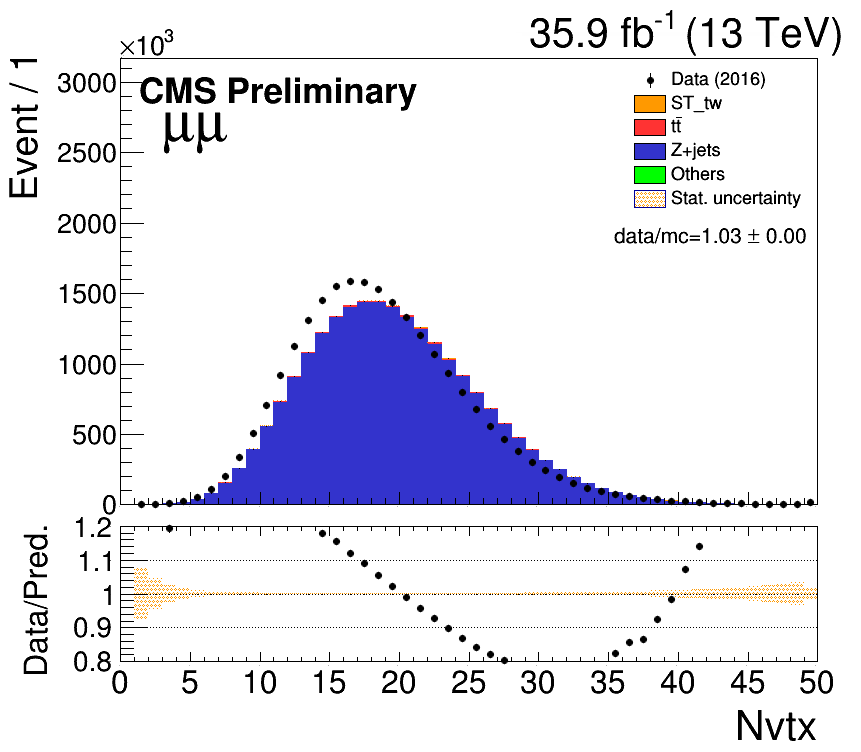
\includegraphics[width=0.32\textwidth]{figures/tW/fig/Step1/mumu_noNvtx/H_pv_n.png}\\
%      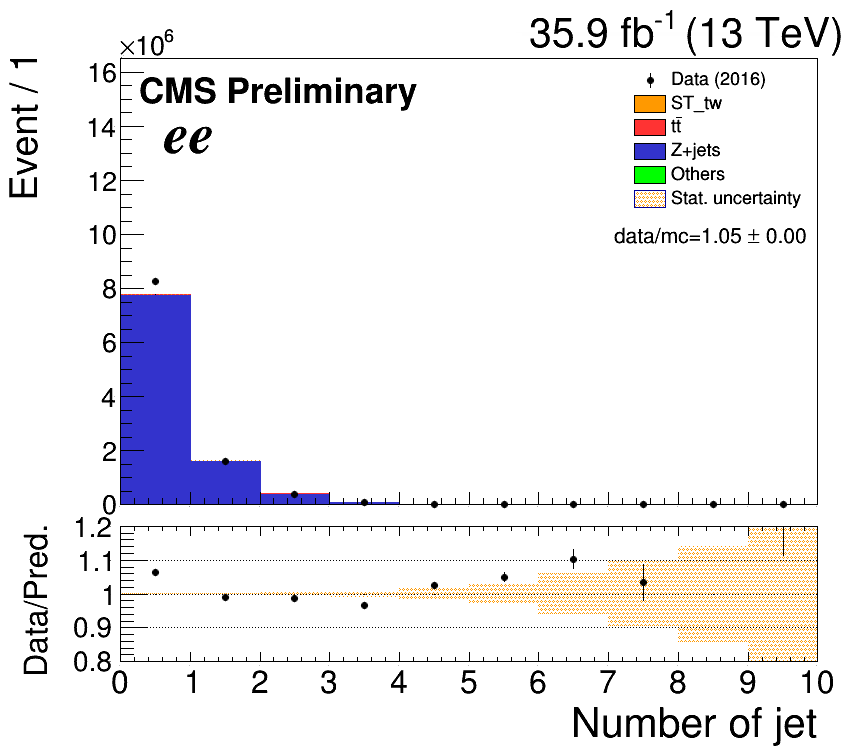
\includegraphics[width=0.32\textwidth]{figures/tW/fig/Step1/ee_noNvtx/H_N_loose_jets.png}&
%      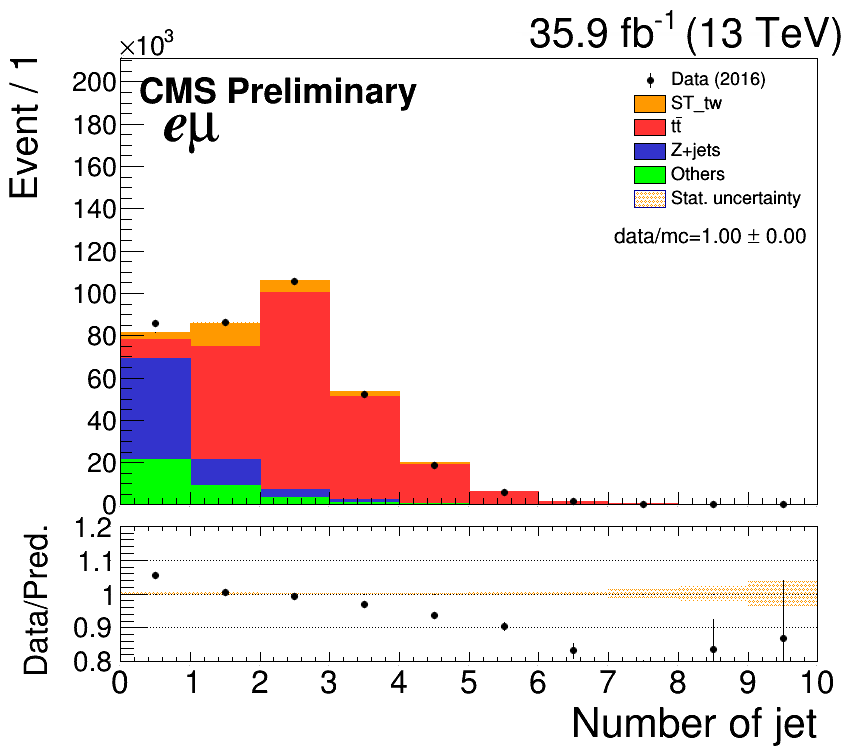
\includegraphics[width=0.32\textwidth]{figures/tW/fig/Step1/emu_noNvtx/H_N_loose_jets.png}&
%      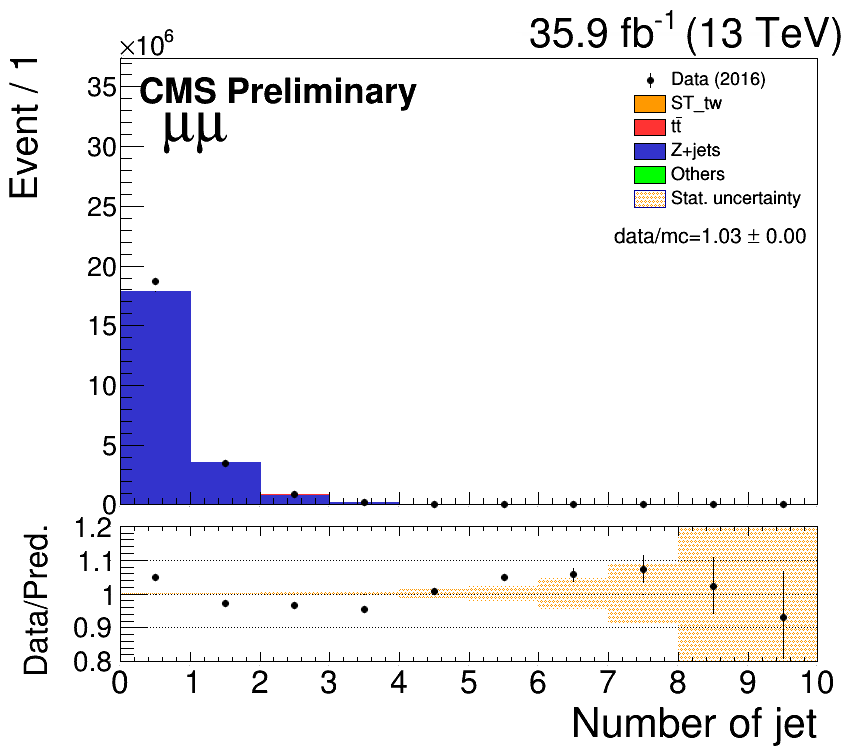
\includegraphics[width=0.32\textwidth]{figures/tW/fig/Step1/mumu_noNvtx/H_N_loose_jets.png}\\
%      \includegraphics[width=0.32\textwidth]{figures/tW/fig/Step1/ee_noNvtx/H_N_b_jets.png}&
%      \includegraphics[width=0.32\textwidth]{figures/tW/fig/Step1/emu_noNvtx/H_N_b_jets.png}&
%      \includegraphics[width=0.32\textwidth]{figures/tW/fig/Step1/mumu_noNvtx/H_N_b_jets.png}\\
%      \includegraphics[width=0.32\textwidth]{figures/tW/fig/Step1/ee_noNvtx/H_njet_bjet.png}&
%      \includegraphics[width=0.32\textwidth]{figures/tW/fig/Step1/emu_noNvtx/H_njet_bjet.png}&
%      \includegraphics[width=0.32\textwidth]{figures/tW/fig/Step1/mumu_noNvtx/H_njet_bjet.png}\\
%    \end{tabular}
%    \caption{The distributions of number of vertices (first row), number of jets (second row), number of b jets (third row) and number of jets-bjets (last row) for $ee$ (left), $e\mu$ (middle) and $\mu\mu$ (right) channels after step 1 (trigger and lepton selections). All backgrounds are estimated from MC.}
%    \label{fig:step1_Nvtx_jet_bjet}
%  \end{center}
%\end{figure}
%
%\begin{figure}[ht]
%  \begin{center}
%    \begin{tabular}{ccc}
%      \includegraphics[width=0.32\textwidth]{fig/EventSelection/_EE_80_step1_T2/EE_80_step1_T2_hratio_jet_leading_pt.png}&
%      \includegraphics[width=0.32\textwidth]{fig/EventSelection/_EMu_80_step1_T2/EMu_80_step1_T2_hratio_jet_leading_pt.png}&
%      \includegraphics[width=0.32\textwidth]{fig/EventSelection/_MuMu_80_step1_T2/MuMu_80_step1_T2_hratio_jet_leading_pt.png}\\
%      \includegraphics[width=0.32\textwidth]{fig/EventSelection/_EE_80_step1_T2/EE_80_step1_T2_hratio_jet_leading_eta.png}&
%      \includegraphics[width=0.32\textwidth]{fig/EventSelection/_EMu_80_step1_T2/EMu_80_step1_T2_hratio_jet_leading_eta.png}&
%      \includegraphics[width=0.32\textwidth]{fig/EventSelection/_MuMu_80_step1_T2/MuMu_80_step1_T2_hratio_jet_leading_eta.png}\\
%      \includegraphics[width=0.32\textwidth]{fig/EventSelection/_EE_80_step1_T2/EE_80_step1_T2_hratio_jet_leading_CSV.png}&
%      \includegraphics[width=0.32\textwidth]{fig/EventSelection/_EMu_80_step1_T2/EMu_80_step1_T2_hratio_jet_leading_CSV.png}&
%      \includegraphics[width=0.32\textwidth]{fig/EventSelection/_MuMu_80_step1_T2/MuMu_80_step1_T2_hratio_jet_leading_CSV.png}\\
%    \end{tabular}
%    \caption{The distributions of pt (first row), $\eta$ (second row) and csv discriminat (third row) of leading jet for $ee$ (left), $e\mu$ (middle) and $\mu\mu$ (right) channels after step 1 (trigger and lepton selections). All backgrounds are estimated from MC.}
%    \label{fig:step1_leading_jet_info}
%  \end{center}
%\end{figure}
%
%\begin{figure}[ht]
%  \begin{center}
%    \begin{tabular}{ccc}
%      \includegraphics[width=0.32\textwidth]{fig/EventSelection/_EE_80_step1_T2/EE_80_step1_T2_hratio_jet_sub_leading_pt.png}&
%      \includegraphics[width=0.32\textwidth]{fig/EventSelection/_EMu_80_step1_T2/EMu_80_step1_T2_hratio_jet_sub_leading_pt.png}&
%      \includegraphics[width=0.32\textwidth]{fig/EventSelection/_MuMu_80_step1_T2/MuMu_80_step1_T2_hratio_jet_sub_leading_pt.png}\\
%      \includegraphics[width=0.32\textwidth]{fig/EventSelection/_EE_80_step1_T2/EE_80_step1_T2_hratio_jet_sub_leading_eta.png}&
%      \includegraphics[width=0.32\textwidth]{fig/EventSelection/_EMu_80_step1_T2/EMu_80_step1_T2_hratio_jet_sub_leading_eta.png}&
%      \includegraphics[width=0.32\textwidth]{fig/EventSelection/_MuMu_80_step1_T2/MuMu_80_step1_T2_hratio_jet_sub_leading_eta.png}\\
%      \includegraphics[width=0.32\textwidth]{fig/EventSelection/_EE_80_step1_T2/EE_80_step1_T2_hratio_jet_sub_leading_CSV.png}&
%      \includegraphics[width=0.32\textwidth]{fig/EventSelection/_EMu_80_step1_T2/EMu_80_step1_T2_hratio_jet_sub_leading_CSV.png}&
%      \includegraphics[width=0.32\textwidth]{fig/EventSelection/_MuMu_80_step1_T2/MuMu_80_step1_T2_hratio_jet_sub_leading_CSV.png}\\
%    \end{tabular}
%    \caption{The distributions of pt (first row), $\eta$ (second row) and csv discriminat (third row) of sub-leading jet for $ee$ (left), $e\mu$ (middle) and $\mu\mu$ (right) channels after step 1 (trigger and lepton selections). All backgrounds are estimated from MC.}
%    \label{fig:step1_subleading_jet_info}
%  \end{center}
%\end{figure}
